\documentclass[11pt]{article}
\usepackage[a4paper,margin=1in]{geometry}
\usepackage{amsmath, amssymb, bm}
\usepackage{graphicx}
\usepackage{booktabs}
\usepackage{adjustbox}
\usepackage{longtable}
\usepackage[numbers,sort&compress]{natbib}
\usepackage{hyperref}
\usepackage{mathtools}
\usepackage{enumitem}

\usepackage[section]{placeins}
\setcounter{topnumber}{2}
\setcounter{bottomnumber}{2}
\setcounter{totalnumber}{4}
\renewcommand{\topfraction}{0.95}
\renewcommand{\bottomfraction}{0.95}
\renewcommand{\textfraction}{0.05}
\renewcommand{\floatpagefraction}{0.85}

\newcommand{\LABone}{LAB$_1$}
\newcommand{\LABtwo}{LAB$_2$}
\newcommand{\LABthree}{LAB$_3$}
\newcommand{\LAB}{LAB$_1$--LAB$_3$}
\newcommand{\StdTableFont}{\footnotesize}
\newcommand{\ManuscriptTitle}{Stable and recurrent deformation subspaces preserve pelvic mechanical function across anatomical variability}
\newcommand{\ShortTitle}{Recurrent pelvic deformation subspaces}
\input{../../analysis_outputs/tables/values.tex}
\newcommand{\StdTableInput}[1]{%
  \begingroup
  \setlength{\tabcolsep}{4pt}%
  \resizebox{\linewidth}{!}{\input{#1}}%
  \endgroup
}
\newcommand{\SuppTableInput}[1]{%
  \begingroup
  \footnotesize
  \setlength{\tabcolsep}{4pt}%
  \renewcommand{\arraystretch}{1.05}%
  \noindent\centering
  \begin{adjustbox}{max width=\linewidth}
    \input{#1}%
  \end{adjustbox}
  \par
  \endgroup
}

\begin{document}

\begin{flushleft}
{\LARGE\bfseries \ManuscriptTitle\par}
\vspace{1.5em}
{\normalsize Petr Heny\v{s}$^{1,2}$, Michal Kucha\v{r}$^{5}$, Alexander Mor\'{a}vek$^{5}$, Niels Hammer$^{2,3,4,*}$\par}
\vspace{0.75em}
{\small $^{1}$Institute of New Technologies and Applied Informatics, Faculty of Mechatronics, Informatics and Interdisciplinary Studies, Technical University of Liberec, Liberec, Czech Republic\par}
{\small $^{2}$Division of Macroscopic and Clinical Anatomy, Gottfried Schatz Research Center, Medical University of Graz, Graz, Austria\par}
{\small $^{3}$Department of Orthopedic and Trauma Surgery, University of Leipzig, Leipzig, Germany\par}
{\small $^{4}$Division of Biomechatronics, Fraunhofer Institute for Machine Tools and Forming Technology (IWU), Chemnitz and Dresden, Germany\par}
{\small $^{5}$Department of Anatomy, Faculty of Medicine in Hradec Kr\'{a}lov\'{e}, Charles University, Hradec Kr\'{a}lov\'{e}, Czech Republic\par}
\vspace{0.75em}
{\small $^{*}$Corresponding author\par}
{\small E-mail: \href{mailto:niels.hammer@medunigraz.at}{niels.hammer@medunigraz.at} (NH)\par}
\vspace{0.75em}
{\small \textbf{Short title:} \ShortTitle\par}
\end{flushleft}

\clearpage


% ============================================================
\section*{Abstract}
Human pelvic kinematics must operate across marked variation in ring geometry, inlet and outlet dimensions, and bone mineral distribution.
Yet, population computational biomechanics commonly compares ranked deformation pathways as if identical spectral labels carried identical anatomical meaning across individuals.
Here, we investigate whether pelvic deformation patterns remain attached to individually stable pathways or are preserved within compact recurrent deformation subspaces.
We analyse the linearised stiffness spectrum of $N{=}278$ subject-specific finite-element models assembled on a shared reference domain with individual bony anatomy and CT-derived elasticity.
Across the population cohort, pelvic deformation partitions into two distinct spectral regimes.
Modes~1--3 form a gap-protected low-rank \emph{backbone} that rarely reorders across subjects ($<0.4\%$ label-exchange rate) and governs habitual standing loads.
Higher ranks contain recurrent \emph{clustered} regimes, most prominently an inlet-related 9--10 block present in 54.7\% of individuals.
Within that block, anterior--posterior inlet coupling redistributes between rank labels~9 and~10 when the labels exchange, yet remains consistently high in their shared two-dimensional subspace and is selectively recruited under parturition-motivated proxy loading.
An outlet-related 5--6 block similarly forms an outlet-related subspace with strong biischiadic coupling despite local label instability.
These findings demonstrate that pelvic compliance is organised across spectral scales: low-rank pathways provide a stable mechanical backbone, whereas higher-order anatomical deformation programs are retained within compact recurrent modal subspaces.
More generally, this framework establishes how anatomical coupling can be preserved across skeletal variability without assuming one-to-one conservation of individual spectral labels.

% ============================================================
\section*{Author summary}

Individuals differ substantially in pelvic shape and bone density, yet every human pelvis must transfer body weight during locomotion while preserving internal canal dimensions.
Biomechanical studies typically compare individuals by examining vibration or deformation modes one by one, assuming that each ranked pattern corresponds to the same mechanical behavior in every person.
Using detailed computational finite-element models of 278 human pelves, we tested whether this assumption holds across population anatomy.
We found that everyday standing loads rely on a few dominant, stable deformation patterns (modes~1--3) that maintain consistent rank ordering and strong shape alignment across individuals (median mass-weighted modal assurance criterion to reference $> 0.96$).
In contrast, patterns associated with widening of the pelvic inlet do not remain attached to a single fixed numerical rank.
Instead, this anatomical opening capacity is preserved across recurrent deformation subspaces whose internal mode order can swap between individuals.
Comparing skeletons strictly mode-by-mode can therefore create the false impression of functional disruption when the underlying anatomical capacity is actually preserved.
Our study provides a principled computational approach to compare anatomically variable structures at the level of small groups of cooperating deformation pathways.


% ============================================================
\section{Introduction}
\label{sec:introduction}

Biological load-bearing structures must maintain mechanical competence across individuals that differ substantially in skeletal morphology and tissue distribution.
The human pelvis exemplifies this challenge: it transfers locomotor forces between the spine and lower limbs while preserving birth canal dimensions critical for parturition~\citep{Washburn1960,Gruss2015,HenyssKuchar2025BoneDat}.
A central computational question is how anatomical deformation pathways remain functionally coherent despite wide population variability.

In biological systems, robustness is achieved through the preservation of functional output under perturbation, frequently supported by degeneracy---the capacity of structurally distinct elements to perform overlapping tasks~\citep{Kitano2004,Kitano2007,Whitacre2010,Whitacre2012}.
In structural biomechanics, transmitting body weight or accommodating internal cavity expansion need not rely on an identical, rigid deformation mode in every individual.
Different pelves may achieve equivalent compliance through slightly different deformation pathways within shared subspaces, analogous to motor synergy recruitment across variable musculoskeletal anatomy~\citep{Ting2012}.

Population computational biomechanics, however, frequently compares modal pathways across subjects under the assumption of stable spectral indexing.
This convention conflates three distinct physical objects:
(i)~\emph{anatomical shape}, describing subject-specific geometry;
(ii)~\emph{deformation pathways}, describing physical ring kinematics; and
(iii)~\emph{spectral rank}, which sorts pathways purely by ascending stiffness.
In linearised elasticity, rank ordering is robust only while adjacent eigenvalues remain well separated.
When eigenvalues crowd, minor perturbations in geometry or tissue density rotate eigenvectors and induce label exchange (veering) even while the physically relevant subspace remains unchanged~\citep{Pierre1988,ManconiMace2017,GhoshGhanem2012}.
Assuming one-to-one correspondence between mode rank and biological function across a cohort therefore introduces a severe risk of misinterpreting local label swaps as genuine functional disruption.

The appropriate unit of analysis in crowded spectral regimes is not the isolated eigenmode, but a \emph{compact recurrent subspace}---a low-dimensional, externally separated block that retains a targeted deformation program across subjects.
The pelvic ring offers an ideal anatomical testbed: its compliance is constrained by joint morphology, articular cartilage, and extensive ligamentous networks~\citep{Snijders1993,Vleeming2012,Goode2008}, yet its population-scale modal stability has remained unexplored.

Here, we evaluate the linearised stiffness spectrum of $N{=}278$ CT-derived, subject-specific finite-element models on a common reference domain to address three testable computational questions:
\begin{enumerate}[label=(\roman*)]
  \item \textbf{Rank stability:} Are primary pelvic deformation pathways order-locked across a variable population cohort, or do they reorder systematically?
  \item \textbf{Subspace preservation:} In crowded spectral regimes, do anatomical compliance observables redistribute between mode labels while remaining stable within compact recurrent subspaces?
  \item \textbf{Load-routing selectivity:} Do habitual standing and parturition-motivated proxy loads recruit distinct modal regimes, separating conserved baseline support from flexible higher-order pathways?
\end{enumerate}


% ============================================================
\section{Results}
\label{sec:results}

\subsection{Interpretable deformation pathways preview two distinct organisational scales}
\label{sec:atlas-results}

Before turning to cohort statistics, it was investigated whether the low-order deformation repertoire already reveals where mechanical meaning is stably localised and where it is likely to be preserved only at the level of a small clustered family.
Figure~\ref{fig:modes-atlas} characterises the global deformation of the complete reference pelvis without separating bones or anatomical branches.
Direct fitting of simple kinematic templates to the local strain field leaves 97--99\% of the norm unexplained across all modes, because compliance and strain heavily concentrate in the cartilaginous joints (sacroiliac joints and pubic symphysis), which drowns out global ring deformation and fails to discriminate modes.
To recover the global ring-level character without imposing artificial 1D beam axes on a closed 3D pelvic ring, we evaluate the overall shape change across the entire 3D continuum: infinitesimal rigid-body translation and rotation are first mathematically removed by orthogonal projection, after which the remaining nonrigid displacement field is decomposed into four canonical 3D deformation families (axial tension/compression, bending, transverse shear, and torsion).
Rigid rotation is eliminated upfront and is not a reported deformation category.
Subspace overlap on the irregular geometry is handled via Shapley allocation of the explained squared nonrigid shape norm; unexplained deformation is retained as an explicit residual.
The resulting fractions are descriptive shape fractions conditional on the kinematic dictionary, not strain-energy shares.
The complete mathematical formulation, positive 14-point (degree-4) tetrahedral quadrature, 24-dimensional polynomial dictionary, Gram matrix conditioning, synthetic validation benchmarks, and complete 15-mode quantitative profile tables are detailed in Appendix~E (Tables~E1--E2).
Population stability is tested separately below.

Higher modes raise a different biological question: whether a mechanically interpretable function remains tied to one label or only to a compact family.
The most important case is the 9--10 pair.
Mode~9 typically exhibits an inlet-opening deformation in which the pubic symphysis and the sacral promontory move apart, widening the pelvic ring.
Mode~10 is a near-degenerate partner with an asymmetric field concentrated around the pubic region.
Their close spacing already suggests that inlet-related behaviour may not be consistently attached to one fixed rank label across subjects, even if it remains preserved within the two-dimensional span they share.
For this region of the spectrum, the pair is therefore a more reliable biological interpretive unit than either label alone.

% Full A4 figure page; preserve physical label sizes in the atlas.
\clearpage
\newgeometry{left=10mm,right=10mm,top=8mm,bottom=8mm}
\begin{figure}[p]
  \centering
  \includegraphics[width=182mm,height=220mm,keepaspectratio]{../../analysis_outputs/plos_revision/figures/reference_mode_atlas.pdf}
  \begingroup
  \fontsize{9}{10.5}\selectfont
  \caption{\textbf{Whole-pelvis deformation patterns of reference modes.}
  Anterior (left) and cranial (right) views show displacement magnitude from purple to yellow, scaled to a 50~mm maximum; grey geometry is undeformed.
  Each bar partitions the whole-pelvis nonrigid squared shape norm into fitted axial tension/compression, bending, transverse shear, torsion, and residual.
  Infinitesimal rigid-body translation and rotation are projected out upfront; rigid rotation is not a reported deformation category.
  The decomposition operates in full 3D Cartesian space across the entire pelvic ring without imposing a 1D reference axis.
  Overlapping pattern subspaces are allocated using Shapley values.
  ``Fitted'' reports the percentage of nonrigid shape change explained by the four canonical 3D families.
  All fractions use the complete continuum without bone-wise subdivision and describe kinematic shape change rather than elastic-energy shares.}
  \label{fig:modes-atlas}
  \endgroup
\end{figure}
\clearpage
\restoregeometry

\subsection{Population variability separates an order-locked backbone from recurrent clustered regimes}
\label{sec:spectral-results}

The cohort of $N{=}278$ subjects resolves the spectrum into two regimes: an order-locked low-rank backbone and recurrent higher-rank clustered blocks (Fig.~\ref{fig:spectral-dashboard}, Table~\ref{tab:clusters}).
Modes~1--3 are rarely reordered across the cohort (swap rate $<0.4\%$), whereas higher ranks contain small consecutive gaps and frequent label exchange.
Using a data-driven cluster threshold $\varepsilon_{\rm in}\approx 0.131$ (25th percentile of pooled relative consecutive gaps; see Methods), we detect nine near-degenerate rank clusters above a 3\% prevalence floor.
The most prevalent cluster is rank modes~9--10 (54.7\% of subjects), followed by rank modes~12--15 (41.7\%) and rank modes~5--6 (33.8\%).
No exact numerical degeneracy ($\mathrm{gap}_{\rm in} \le 10^{-6}$) is observed, as expected for a three-dimensional asymmetric anatomical structure without continuous rotational or discrete reflectional symmetries.

Anatomical variability does not destabilise the spectrum uniformly.
Label fragility is concentrated in a small number of compact families, while low-rank order is preserved.
For the dominant 9--10 and 12--15 clusters, median relative internal gaps are small enough that modest perturbations can reverse local ordering.
The clusters nevertheless remain externally separated from neighbouring modes, so they are best interpreted as compact clustered subspaces rather than as a global loss of spectral organisation.
This pattern is consistent with a pelvic system that preserves stable baseline load-transfer pathways while allowing selected higher-rank functions to vary within a limited local repertoire.

Permutation statistics reinforce this interpretation.
Modes~12 and~13 exhibit the highest swap rates, and mode~15 also shows a sizeable unpaired fraction under strict cross-subject pairing, whereas the backbone is essentially fixed in its ordering.
For population computational biology the consequence is concrete: while one-to-one modal comparison is well-conditioned for the low-rank backbone, higher-rank comparisons must accommodate mode mixing and label exchange through subspace representations.

A variability decomposition into shape-only and material-only datasets (Fig.~\ref{fig:spectral-dashboard}C) shows that shape variability accounts for the largest share of the coefficient of variation for modes~1--8, whereas bone-density heterogeneity contributes with increasing relative weight in modes~9--15.
Shape changes alter \emph{how} the spatial density heterogeneity enters the stiffness operator: shape dominates lower modal variance while material heterogeneity contributes increasingly at higher ranks.
This structural reweighting preserves a conserved low-rank backbone while pushing selected higher-rank directions toward clustered, near-degenerate behaviour.

These prevalence estimates are not driven by a few outliers or by the order in which subjects are processed.
Subsampling stability analysis (500 random draws of 80\% cohort size without replacement) yields narrow 95\% stability intervals for the dominant clusters (9--10: 51.8--57.7\%; 12--15: 38.7--45.0\%), confirming that cluster detection is robust to cohort composition. In addition, full subject resampling with replacement ($N{=}278$, 500 replicates) with threshold re-estimation confirms consistent prevalence estimates. Random permutation of subject order leaves cluster prevalence and swap statistics unchanged to machine precision.
The central spectral hierarchy is therefore a cohort-level feature rather than a post-processing artefact.
Additional cluster-mapping, swap, and robustness diagnostics are provided in Appendix~A and Appendix~B.

\begin{figure}[!htbp]
  \centering
  \includegraphics[width=\linewidth,height=0.68\textheight,keepaspectratio]{../../analysis_outputs/plos_revision/figures/spectral_structure.pdf}
  \caption{\textbf{Population variability partitions the stiffness spectrum into an order-locked backbone and clustered higher ranks.}
  \textbf{(A)} Consecutive relative spectral gaps $\mathrm{gap}_{\rm in}(i) = (\lambda_{i+1}-\lambda_i)/\lambda_i$ across the cohort ($N{=}278$); the dashed line marks the data-driven cluster threshold $\varepsilon_{\rm in} \approx 0.131$ (25th percentile).
  \textbf{(B)} Subject fraction exhibiting label exchange (blue) and unpaired pairing failures (grey; $\mathrm{MAC}_{M_0} < 0.05$) per reference label.
  \textbf{(C)} Eigenvalue variability (coefficient of variation, CoV) across the combined cohort (blue), shape-only cohort (orange), and material-only cohort (green).}
  \label{fig:spectral-dashboard}
\end{figure}

\begin{table}[!htbp]
\centering
\caption{\textbf{Recurrent clustered rank blocks detected above the 3\% prevalence floor.}}
\label{tab:clusters}
\StdTableFont
\StdTableInput{../../analysis_outputs/tables/clusters.tex}
\end{table}

\subsection{Clustered subspaces preserve distinct mechanical programs under variability}
\label{sec:subspace-results}

Once individual labels become unstable, the next question is whether the corresponding small recurrent subspaces remain mechanically distinct.
Figure~\ref{fig:subspace-dashboard} shows that several do, when interpreted using invariant-subspace descriptors rather than individual eigenvector labels.
Two basis-invariant outputs were evaluated.
First, Grassmann distance from a reference subject quantifies how much a subspace rotates across the cohort.
Second, canonical coupling to anatomical diameter functionals (AP and ML inlet; biischiadic and bituberous outlet) provides functionally interpretable coordinates inside each clustered block (Methods).

The rank~9--10 subspace shows the strongest inlet-related coupling among the prevalent clusters.
Its median AP-inlet coupling is \BlockNineTenAP\,mm of inlet diameter change per 1\,mm of maximum nodal modal amplitude, making 9--10 the clearest higher-rank inlet-related program in the cohort.
In contrast, the rank~5--6 cluster shows the strongest transverse outlet-related coupling, with median biischiadic widening \BlockFiveSixBIS\,mm/mm and bituberous response \BlockFiveSixBIT\,mm/mm (accompanied by \BlockFiveSixOUTLETAP\,mm/mm for outlet AP dilation; in the 9--10 subspace, biischiadic widening reaches \BlockNineTenBIS\,mm/mm and outlet AP reaches \BlockNineTenOUTLETAP\,mm/mm).
Different clustered subspaces therefore carry different mechanical programs: one is functionally aligned with the inlet, another with the outlet.

The four-dimensional 12--15 block illustrates a third regime.
It has high prevalence, small internal gaps, and a richer pattern of within-block mixing than a simple two-mode exchange.
Its canonical coupling structure is more diffuse than in 9--10 or 5--6, consistent with it representing a broader, higher-order reserve rather than a single sharply interpretable program.
Furthermore, because spectral eigensolves were truncated at $N_{\rm ev}=15$, external separation of this upper block on the right cannot be determined without higher eigenvalues; we therefore treat 12--15 as a diffuse higher-rank regime bounded by modal truncation.
Not every recurrent cluster corresponds to one clean anatomical function.
This heterogeneity is itself biologically informative: the framework separates compact, functionally specific blocks from mixed higher-rank families, and the former are the clearest targets for single-function biological interpretation.


Subspace orientation in the ambient displacement space (quantified by the Grassmann distance $d_G$, which is strictly invariant to internal basis rotations) also varies systematically with sex.
The largest contrast is observed for the 9--10 block, indicating that female and male anatomies orient this two-dimensional inlet subspace along slightly different directions in $\mathbb{R}^n$.
This qualifies how clustered behaviour is distributed across the population without altering the central point: recurrent clustered subspaces retain distinct mechanical meanings across sexes despite modest differences in their ambient subspace orientation.

\begin{figure}[!htbp]
  \centering
  \includegraphics[width=\linewidth]{../../analysis_outputs/plos_revision/figures/functional_coupling.pdf}
  \caption{\textbf{Anatomical diameter coupling across recurrent clustered modal subspaces.}
  Canonical coupling scores (mm diameter change per mm maximum nodal displacement) for the five most prevalent rank blocks across the cohort ($N{=}278$):
  \textbf{(A)}~anteroposterior (AP) inlet,
  \textbf{(B)}~mediolateral (ML) inlet,
  \textbf{(C)}~biischiadic outlet, and
  \textbf{(D)}~bituberous outlet.
  Boxes indicate median and interquartile range (IQR); whiskers extend to $1.5\times\mathrm{IQR}$.}
  \label{fig:subspace-dashboard}
\end{figure}

\subsection{Subspace-level preservation is more stable than fixed labels in clustered regimes}
\label{sec:label-results}

A direct consequence of this framing follows: in a clustered regime, function should be preserved more stably at the scale of the subspace than at the scale of its individual labels.
This hypothesis was tested for the most prevalent cluster, rank modes~9--10 (Fig.~\ref{fig:label-stability}).

Among subjects within the 9--10 cluster ($n{=}\ClusterMemberN$), AP-inlet coupling attached to \emph{rank mode~9} is high when labels do not swap ($n{=}\ClusterNoSwapN$) and low when they do ($n{=}\ClusterSwapN$) (median \RankNineNo\ vs.\ \RankNineYes\,mm/mm; difference \RankNineDifference\,mm/mm, 95\% CI [\RankNineLow, \RankNineHigh], $p = \RankNinePformatted$, rank-biserial $r_{\rm rb} = \RankNineRankBiserial$).
The complementary pattern appears for \emph{rank mode~10} (median \RankTenNo\ vs.\ \RankTenYes\,mm/mm; difference $+$\RankTenDifference\,mm/mm, 95\% CI [\RankTenLow, \RankTenHigh], $p = \RankTenPformatted$, $r_{\rm rb} = \RankTenRankBiserial$).
Label-level coupling therefore redistributes decisively between the two rank indices, not because the inlet-related signal disappears, but because it shifts inside the same two-dimensional block while the solver labels exchange ($p < 10^{-21}$ for both modes).

By contrast, the \emph{subspace-level} AP capacity of the 9--10 block remains substantial across both groups (basis-invariant single-functional capacity $\widehat\kappa_{\rm AP}$: median \ScalarAPNo\ vs.\ \ScalarAPYes\,mm/mm; difference \ScalarAPDifference\,mm/mm, 95\% CI [\ScalarAPLow, \ScalarAPHigh], ratio \ScalarAPRatio, $p = \ScalarAPPval$, $r_{\rm rb} = \ScalarAPRankBiserial$; companion joint-SVD score: median \PairAPNo\ vs.\ \PairAPYes\,mm/mm, difference \PairAPDifference\,mm/mm, 95\% CI [\PairAPLow, \PairAPHigh], $p = \PairAPPval$).
In sharp contrast to the massive, statistically decisive redistribution seen at the single-mode level ($p < 10^{-21}$), the subspace-level capacity exhibits only modest descriptive variation between non-swapped and swapped groups (difference \ScalarAPDifference\,mm/mm, 95\% CI [\ScalarAPLow, \ScalarAPHigh], $p = \ScalarAPPval$).
Across the entire unselected cohort ($N{=}\CohortN$; \CohortNoSwapN\ no-exchange vs.\ \CohortSwapN\ exchange), rank~9 coupling shifts by \CohortRankNineDifference\,mm/mm ($p = \CohortRankNinePformatted$) and rank~10 shifts by $+$\CohortRankTenDifference\,mm/mm ($p = \CohortRankTenPformatted$), whereas subspace-level single-functional capacity differs by only \CohortScalarAPDifference\,mm/mm (95\% CI [\CohortScalarAPLow, \CohortScalarAPHigh], $p = \CohortScalarAPPformatted$, non-significant descriptive contrast).
What becomes unstable is the attachment of the function to one rank index rather than another, not the anatomical capability itself.
Across-subject comparisons of higher-order clustered modes phrased as though ``mode~9'' or ``mode~10'' were fixed entities across the cohort can therefore be misleading.
For this regime, the biologically meaningful unit is a compact recurrent subspace---here the shared 9--10 block.

Load routing reinforces the same conclusion (Fig.~\ref{fig:tradeoff}).
The 9--10 exchange is primarily a labelling instability with quantitative tuning, not a loss of the inlet-related program.
Subspace rotation and the internal 9--10 gap vary across subjects, AP coupling shifts modestly with swap status, and the throughput of the 9--10 block under \LAB\ depends on morphology in a phase-specific way.
For \LABone, block throughput decreases with larger AP inlet diameter ($\rho_s{=}{-}0.48$, $p{=}4.3\times10^{-17}$), whereas \LABtwo\ and \LABthree\ show weaker and differently signed trends.
These patterns support the interpretation that inlet-related mechanics remains associated with the 9--10 subspace even as anatomical variability redistributes its basis representation and modulates its phase-specific amplitude.

\begin{figure}[!htbp]
  \centering
  \includegraphics[width=\linewidth]{../../analysis_outputs/plos_revision/figures/label_stability.pdf}
  \caption{\textbf{Inlet coupling redistributes between rank labels within the stable 9--10 subspace.}
  Anteroposterior (AP) inlet coupling for rank mode~9 \textbf{(A)}, rank mode~10 \textbf{(B)}, and the basis-invariant single-functional AP capacity of the two-dimensional 9--10 subspace \textbf{(C)}, stratified by $9\rightleftarrows 10$ label-exchange status.
  Points represent individual cluster-member subjects ($n{=}\ClusterMemberN$; no-exchange $n{=}\ClusterNoSwapN$, exchange $n{=}\ClusterSwapN$; male in blue, $n{=}\ClusterMaleN$; female in yellow, $n{=}\ClusterFemaleN$).
  Horizontal lines indicate medians; boxes indicate interquartile range; whiskers indicate $1.5\times\mathrm{IQR}$.
  Coupling is expressed as diameter change per millimetre of maximum nodal displacement.}
  \label{fig:label-stability}
\end{figure}

\begin{figure}[!htbp]
  \centering
  \includegraphics[width=\linewidth]{../../analysis_outputs/plos_revision/figures/routing_associations.pdf}
  \caption{\textbf{Morphology and loading modulate recruitment of the 9--10 modal block.}
  \textbf{(A--C)} Modal strain-energy fraction carried by the 9--10 block as a function of AP inlet diameter for \LABone\ (bilateral internal ring expansion), \LABtwo\ (ischial distraction), and \LABthree\ (outlet distraction).
  Blue dots and dashed lines indicate males; yellow dots and dashed lines indicate females.
  \textbf{(D)} Basis-invariant single-functional AP-inlet capacity of the 9--10 subspace stratified jointly by sex and label-exchange status (M/no, F/no, M/yes, F/yes). Boxes show median and IQR; whiskers extend to $1.5\times\mathrm{IQR}$.}
  \label{fig:tradeoff}
\end{figure}

\subsection{Standing and proxy loads distinguish backbone-dominated routing from higher-rank recruitment}
\label{sec:load-results}

Load routing reflects the same separation between conserved baseline support and selective higher-rank recruitment (Fig.~\ref{fig:fractions-panel}, Table~\ref{tab:dominant-sets}).
Standing is dominated by the gap-protected low-rank backbone.
Symmetric two-leg standing (SP2leg) is concentrated in mode~2 alone, which carries about 84.5\% of the retained modal strain energy; single-leg standing (SP1leg) distributes energy across the full rotational triad (modes~1--3), reaching a top-3 cumulative share of about 92.1\%.
Within this linear setting, habitual load transfer therefore operates through a small, stable, low-dimensional program.

The proxy load family recruits higher-rank modes.
\LABone, bilateral mediolateral internal ring expansion ($\pm 400$\,N outward), preferentially engages the rank~9--10 inlet-related subspace, which carries a mean energy share of about 0.51 and is led by the inlet-opening mode.
\LABtwo, bilateral ischial-tuberosity distraction, reroutes energy into the mid-rank block at modes~4--8, where the 5--6 outlet-related pair becomes especially important.
\LABthree, anteroposterior outlet distraction, is hybrid, retaining sizeable low-rank contributions while also recruiting mid-rank and 9--10 pathways.
Different loading geometries recruit different parts of the higher-rank spectrum, while continuing to use the backbone as common support.

Among the recurrent clustered regimes, 9--10 remains the clearest case because it combines high cohort prevalence, clear inlet-related interpretation, direct label-versus-subspace evidence (Fig.~\ref{fig:label-stability}), and substantial recruitment under \LABone.
The 5--6 pair remains an outlet-related secondary contrast under \LABtwo, whereas 12--15 is common but behaves, under the present load family, as a mixed higher-rank reserve rather than a single dominant pathway.
Additional load-specificity and sex-stratified summaries are reported in Appendix~B and Appendix~C.

These are linear comparative proxy loads, not simulations of labour.
They do not model fetal contact, tissue remodelling, hormone-dependent softening, or nonlinear late-stage birth mechanics.
Their value is comparative: they reveal which deformation programs are preferentially recruited under different loading geometries, not whether the model can predict clinical childbirth outcomes.

\begin{figure}[!htbp]
  \centering
  \includegraphics[width=\linewidth]{../../analysis_outputs/plos_revision/figures/load_routing.pdf}
  \caption{\textbf{Standing and proxy childbirth loads recruit distinct modal regimes.}
  \textbf{(A)} Heatmap of mean retained modal strain-energy share across the 15 lowest solver ranks for standing (SP2leg, SP1leg) and proxy childbirth loads (\LABone--\LABthree).
  \textbf{(B)} Partition of retained modal strain energy across functional blocks: low-rank backbone (modes~1--3; blue), mid-rank regime (modes~4--8; orange), inlet cluster (modes~9--10; green), and higher-rank reserve (modes~11--15; purple). Standing concentrates in the backbone, whereas proxy loads recruit higher ranks in a task-specific pattern.}
  \label{fig:fractions-panel}
\end{figure}

\begin{table}[!htbp]
\centering
\caption{\textbf{Dominant mode sets for the standing and proxy loading cases.}
$N_{80}$ denotes the smallest set of modes required to reach 80\% cumulative mean energy fraction.}
\label{tab:dominant-sets}
\StdTableFont
\StdTableInput{../../analysis_outputs/tables/mode_activation_dominant_sets.tex}
\end{table}

\subsection{Load-routing overlap distinguishes shared backbone support from selective clustered recruitment}
\label{sec:overlap-results}

Overlap analysis confirms that shared low-rank support and task-specific higher-rank routing are not the same thing.
Both standing cases remain backbone-dominated, yet they are not identical: SP2leg reaches 80\% cumulative throughput with mode~2 alone, whereas SP1leg requires the full triad modes~1--3.
Among the proxy loads, \LABone\ is distinguished by its emphasis on the 9--10 inlet-related subspace, whereas \LABtwo\ and \LABthree\ share greater mid-rank content, which clarifies why the 5--6 pair is an outlet-related secondary result rather than a side observation.
Shared dominant modes and shared full routing profiles are therefore complementary but inequivalent descriptors.
Population-scale spectral structure thus separates a conserved low-rank backbone from a selectively recruited higher-rank repertoire whose function is typically more stable at the subspace level than at the level of individual labels.
Detailed pairwise overlap values are provided in Appendix~C.

\subsection{A minimal two-mode model reproduces the observed label--subspace dissociation}
\label{sec:toy-results}

The organisation observed in the pelvic cohort admits a compact analytical interpretation in terms of the two- and three-degree-of-freedom models of Sec.~\ref{sec:toy-methods}.
Fig.~\ref{fig:toy} shows a stochastic cohort in which a morphology coordinate $\mu$ modulates the detuning of a clustered pair on top of a gap-protected backbone, with additional cohort-level nuisance variability introduced through a compliant hidden pathway of scale $\eta$.
The three model behaviours mirror the three empirical findings of the preceding subsections.
First, the backbone mode keeps a stable rank across all subjects and all values of $\mu$ (Fig.~\ref{fig:toy}A), matching the order-locked behaviour of modes~1--3 in the FE cohort.
Second, as $\mu$ crosses the near-degenerate zone, the two cluster labels exchange their coupling to an inlet-like functional while the two-dimensional cluster subspace continues to carry the function (Fig.~\ref{fig:toy}B), reproducing the label-versus-subspace split documented for the 9--10 pair (Fig.~\ref{fig:label-stability}).
Third, a standing-like load routes almost entirely through the backbone, while a task-like load recruits the clustered block, with the label-level split between its two modes moving between subjects but the block-level recruitment staying high (Fig.~\ref{fig:toy}C), mirroring the backbone-versus-higher-rank contrast in the SP2leg/SP1leg and \LAB\ load cases.
Increasing the hidden-pathway variability scale~$\eta$ at fixed morphology broadens the label-swap rate while leaving subspace coupling and task routing essentially unchanged (Fig.~\ref{fig:toy}D), illustrating how cohort-level nuisance variability expected from unmodelled tissue heterogeneity can change which mode carries the function without changing whether the function is carried.
The two-dimensional cluster in the toy model plays the same role as $\mathrm{span}(Q_s)$ in the FE framework, and the morphology coordinate~$\mu$ illustrates how a continuous anatomical shift can detune eigenvalues across an avoided crossing (minimum-gap) veering region.
Importantly, our empirical permutation null test across the patient cohort (Table~A6) did not show statistically significant localisation of label exchange along the AP diameter axis alone (all permutations yielded empirical $p > 0.05$, designated ``NO'' across test cases).
This negative null test is scientifically revealing: it demonstrates that the toy model serves as a conceptual and mechanistic illustration of parameter-driven detuning and eigenvalue veering across a near-degenerate zone, rather than proof of one-dimensional anatomical causality.
In real pelvic anatomy, mode exchange is governed by the concerted, multi-dimensional variation of the complete 3D ring geometry and boundary restraints, not by an isolated 1D diameter.
This minimal model therefore formalises why the interpretive unit must shift from \emph{mode label} to \emph{cluster subspace} precisely in the regime in which spectral gaps collapse, and why this shift preserves anatomical deformation specificity without requiring one-dimensional geometric determinism.


\begin{figure}[!htbp]
  \centering
  \includegraphics[width=\linewidth]{../../analysis_outputs/plos_revision/figures/toy_model.pdf}
  \caption{\textbf{Minimal analytical model illustrates label exchange within a stable subspace.}
  A stochastic cohort of the analytical model with morphology parameter~$\mu$ and hidden-pathway scale~$\eta$.
  \textbf{(A)} Spectrum: a separated backbone mode and a nearby eigenvalue pair undergoing near-degeneracy around $\mu \approx 0$.
  \textbf{(B)} Functional projection: coupling shifts between individual rank labels across the transition zone while total coupling within the pair remains high.
  \textbf{(C)} Load routing: standing-like load concentrates in the backbone, whereas task-like load recruits the clustered block with a variable between-label split.
  \textbf{(D)} Effect of hidden-pathway variability scale~$\eta$: label-exchange rate increases with~$\eta$, whereas subspace coupling and task routing remain stable.
  Model derivations and simulation parameters are detailed in Methods.}
  \label{fig:toy}
\end{figure}

% ============================================================
\section{Discussion}
\label{sec:discussion}

\subsection*{Subspace preservation resolves the tension between anatomical variability and functional stability}

This pelvic cohort demonstrates that anatomical deformation programs can remain robust across substantial skeletal variability without requiring rigid one-to-one conservation of individual spectral ranks.
Habitual load transfer is concentrated in a low-rank backbone, whereas higher-order anatomical deformations are preserved within compact recurrent subspaces.
The essential biological insight is not merely that spectral labels can become unstable, but that anatomical variation redistributes deformation within a compact local repertoire while preserving the anatomical capability itself.

This distinction separates three objects often conflated in comparative biomechanics: anatomical shape, deformation pathway, and spectral rank.
Shape varies continuously across individuals; deformation pathways describe physical kinematic motions of the ring; and spectral rank merely sorts these pathways by ascending stiffness.
When analysis is restricted to fixed eigenvector ranks, subject-to-subject variability can easily be mistaken for functional loss or chaotic instability.
By evaluating the system through invariant modal subspaces, we demonstrate that mechanical meaning is not lost; rather, the appropriate unit of biological organisation shifts from the isolated eigenmode to a compact, recurrent subspace.

A concrete practical implication follows for population biomechanics: when comparing inlet compliance across individuals using rank mode~9 alone, subjects who undergo a $9\rightleftarrows 10$ label exchange (\ClusterSwapN\ of \ClusterMemberN\ cluster members, $37.5\%$) exhibit an apparent collapse of AP-inlet coupling (from median \RankNineNo\ down to \RankNineYes\,mm/mm, an apparent drop of $\approx 69\%$), falsely suggesting a severe impairment of ring dilation.
In reality, evaluating the shared two-dimensional 9--10 subspace reveals that the anatomical opening capability is substantially more stable across both groups (basis-invariant single-functional capacity: \ScalarAPNo\ vs.\ \ScalarAPYes\,mm/mm; joint canonical coupling: \PairAPNo\ vs.\ \PairAPYes\,mm/mm).
Adopting a subspace framework directly resolves false-negative biomechanical classifications that arise purely from mode tracking across near-degenerate regimes.

\subsection*{Functional organization across spectral scales: Conserved backbone versus flexible higher-rank reserves}

The low-rank backbone represents the order-locked regime.
Modes~1--3 remain spectrally separated, rarely reorder across the cohort ($<0.4\%$ swap rate), and dominate habitual standing loads (carrying $84.5\%$ of retained modal strain energy in symmetric two-leg stance and $92.0\%$ across the triad in single-leg stance).
Because eigenvalues $\lambda_k$ quantify modal stiffness, these lowest-eigenvalue modes represent the highest-compliance baseline deformation pathways of the pelvic ring.
Within the present linear framework, this supports the view that the low-order kinematic pathways of the pelvic ring are governed by a conserved, mechanically accessible baseline program.
We do not infer an evolutionary optimisation principle from these data alone, but the result is physically consistent with biological robustness being anchored in a compact, gap-protected foundation~\citep{Kitano2007,Whitacre2010}.

The higher ranks reveal an organisation characterised by recurrent clustered blocks.
The rank~9--10 pair exemplifies this regime: inlet-related dilation is not reliably attached to a single rank label across the cohort, but the shared two-dimensional subspace retains substantial AP-inlet coupling and is strongly recruited under parturition-aligned proxy loads (\LABone).
Rather than positing an unverified evolutionary selection for structural degeneracy, our results provide a physical interpretation compatible with mechanics: in complex ring structures with near-degenerate eigenvalue spectra, spectral clustering arises naturally as a consequence of three-dimensional ring geometry and material heterogeneity, enabling structurally distinct internal pathways to provide equivalent functional deformations without requiring exact mathematical symmetry~\citep{Whitacre2010,Whitacre2012,EdelmanGally2001}.
In parallel, the 5--6 block forms an outlet-related subspace with strong biischiadic coupling, whereas the broader 12--15 family behaves as a higher-order reserve with diffuse canonical coupling.

\subsection*{Implications for the obstetrical dilemma and population biomechanics}

The human pelvic ring has long been studied through the framework of the ``obstetrical dilemma''~\citep{Washburn1960,Gruss2015}, which posits an evolutionary tension between the structural rigidity necessary for efficient bipedal locomotion and the internal dimensions required for the birth of large-brained neonates.
Our modal analysis provides a mechanistic perspective on how these competing functional demands are partitioned across spectral scales.
Locomotor loads (such as standing and single-leg support) are absorbed primarily by the low-eigenvalue baseline modes (modes~1--3), which provide the natural compliance pathways for habitual weight-bearing.
Conversely, parturition-aligned loading conditions do not simply engage this baseline triad; instead, they selectively recruit higher-rank clustered modes---most prominently the inlet-dilating 9--10 subspace---whose kinematically specialized deformation fields directly widen birth-canal diameters.

Furthermore, our minimal analytical model (Sec.~\ref{sec:toy-results}) demonstrates that cohort-level nuisance variability---such as that arising from unmodelled ligamentous laxity, pelvic floor compliance, or subtle morphological detuning---can easily induce label veering between nearby modes.
Crucially, as shown in Fig.~\ref{fig:toy}D, increasing the scale of hidden-pathway variability ($\eta$) accelerates the rate of label exchange between individual modes without degrading subspace-level functional coupling or load throughput.
This indicates that the pelvic ring can tolerate individual-level variations in soft-tissue stiffness and shape while reliably preserving substantial capacity for inlet and outlet expansion.


\subsection*{Methodological scope, physiological limitations, and future directions}

What generalises from this study is the logic for testing robustness, not the exact pelvic cluster layout.
Combining spectral gap structure, subspace comparison via Grassmann distance, anatomically defined functionals, and modal strain-energy routing makes it possible to evaluate whether function is preserved through stable individual pathways or through stable subspaces in any anatomically variable, load-bearing biological system.
The specific rank partition observed here should not be transferred uncritically to other skeletal assemblies or altered physiological states, nor should every recurrent cluster be assumed to map cleanly onto a single anatomical degree of freedom.

Several limitations bound the physiological interpretation of these findings.
First, the present analysis is linearised, evaluating the initial tangent stiffness operator of the pelvic ring.
Childbirth is a complex, contact-driven, large-deformation process accompanied by progressive viscoelastic relaxation and hormone-induced ligament softening (principally via relaxin and progesterone)~\citep{BiomechPregnancy2022,ChenGrimm2021,Almeida2024Uterus,Vleeming2012}.
The linear modal spectrum characterises the deformation repertoire immediately available before large-scale joint separation occurs; it does not simulate the descent of the fetal head or predict clinical labour outcomes~\citep{BonetWood1997}.
Second, the cohort was assembled from clinical CT scans with a mean subject age of $\approx 54$~years, which may not fully represent the pelvic morphology of primiparous women.
Third, while baseline cartilage and ligament stiffnesses were calibrated against literature values, subject-specific ligament properties were not available.
Our material uncertainty analysis employs first-order Taylor series propagation rather than full non-linear Monte Carlo sampling, which is computationally prohibitive across 278 high-resolution 3D finite-element meshes; while first-order propagation accurately reflects localized sensitivity and covariance-aware gap variances, it does not capture higher-order non-linear parameter interactions.
Nonetheless, our sensitivity analyses (Appendix~D) confirm that realistic material uncertainty raises overall spectral variability without reorganising the underlying gap architecture or dismantling the clustered regimes.
Extending this subspace framework to include geometrically nonlinear deformation, full stochastic sampling, and individualised soft-tissue kinematics represents a promising direction for future population biomechanics.

% ============================================================
\section{Materials and methods}
\label{sec:methods}

The Methods below state the computational framework in self-contained form.
The core objects are (i)~a pullback-assembled linear-elasticity problem on a shared reference domain, (ii)~a subject-specific generalised eigenproblem, (iii)~a cross-subject pairing on a common mass metric, (iv)~a gap-based detector for recurrent clustered regimes, (v)~invariant-subspace comparison via principal angles and the Grassmann distance, and (vi)~basis-invariant anatomical functionals that supply physically interpretable coordinates inside otherwise ambiguous clustered subspaces.
Wherever possible, we use notation that separates three distinct objects: the solver \emph{rank} index~$j$ (the $j$-th smallest eigenvalue for each subject), the paired \emph{reference} label $i = \pi_s^{-1}(j)$ (a cross-subject identifier via inverse assignment), and the \emph{anatomical} functional~$\ell$ (a linear observable defined on the template mesh).


\subsection{Ethics statement}

This study analysed a previously published, anonymised imaging-derived dataset and its associated precomputed finite-element repository (BoneDat)~\citep{HenyssKuchar2025BoneDat}.
No new human imaging or interventions were performed for this work.
According to the BoneDat descriptor, use of the source imaging data was approved by the Ethics Committee of the University Hospital Hradec Kralove (reference 202411IO3P) with waiver of informed consent; we refer readers to the dataset publication for full ethical and governance details.

\subsection{Cohort and geometry normalisation}
\label{sec:cohort}

We analysed a precomputed set of $N{=}278$ CT-derived pelvic finite-element models assembled on a common reference domain ($n_F{=}150$, $n_M{=}128$; age 16--91~yr, mean $54\pm19$).
No new cohort was recruited.
The source repository provides standardised pelvic geometries suitable for in silico analysis~\citep{HenyssKuchar2025BoneDat}.
The reference pelvic domain $\Omega_{\rm ref}$ was discretized using a conforming volumetric mesh comprising $\approx 410\,000$ linear four-node tetrahedral elements (Lagrange $P_1$, totaling $\approx 1.2\times 10^6$ displacement degrees of freedom), with conforming interfaces between the bony segments (sacrum, left and right ossa coxae) and the joint cartilage domains (bilateral sacroiliac articular cartilage and the pubic symphysis disc).
A diffeomorphic registration $\chi_s: \Omega_{\rm ref}\to\Omega_s$ with deformation gradient $F_s(X)=\nabla_X\chi_s(X)$ and Jacobian $J_s=\det F_s>0$ maps the template domain $\Omega_{\rm ref}$ onto each subject domain $\Omega_s$.
The pipeline standardises bulk pelvic size so that the main population analysis isolates shape-driven and material-driven variability rather than absolute scale.
Figure~\ref{fig:model-setup} summarises the anatomical dimensions, ligament representation, and boundary-condition layout used to define the pelvic models analysed here.


\begin{figure}[!htbp]
  \centering
  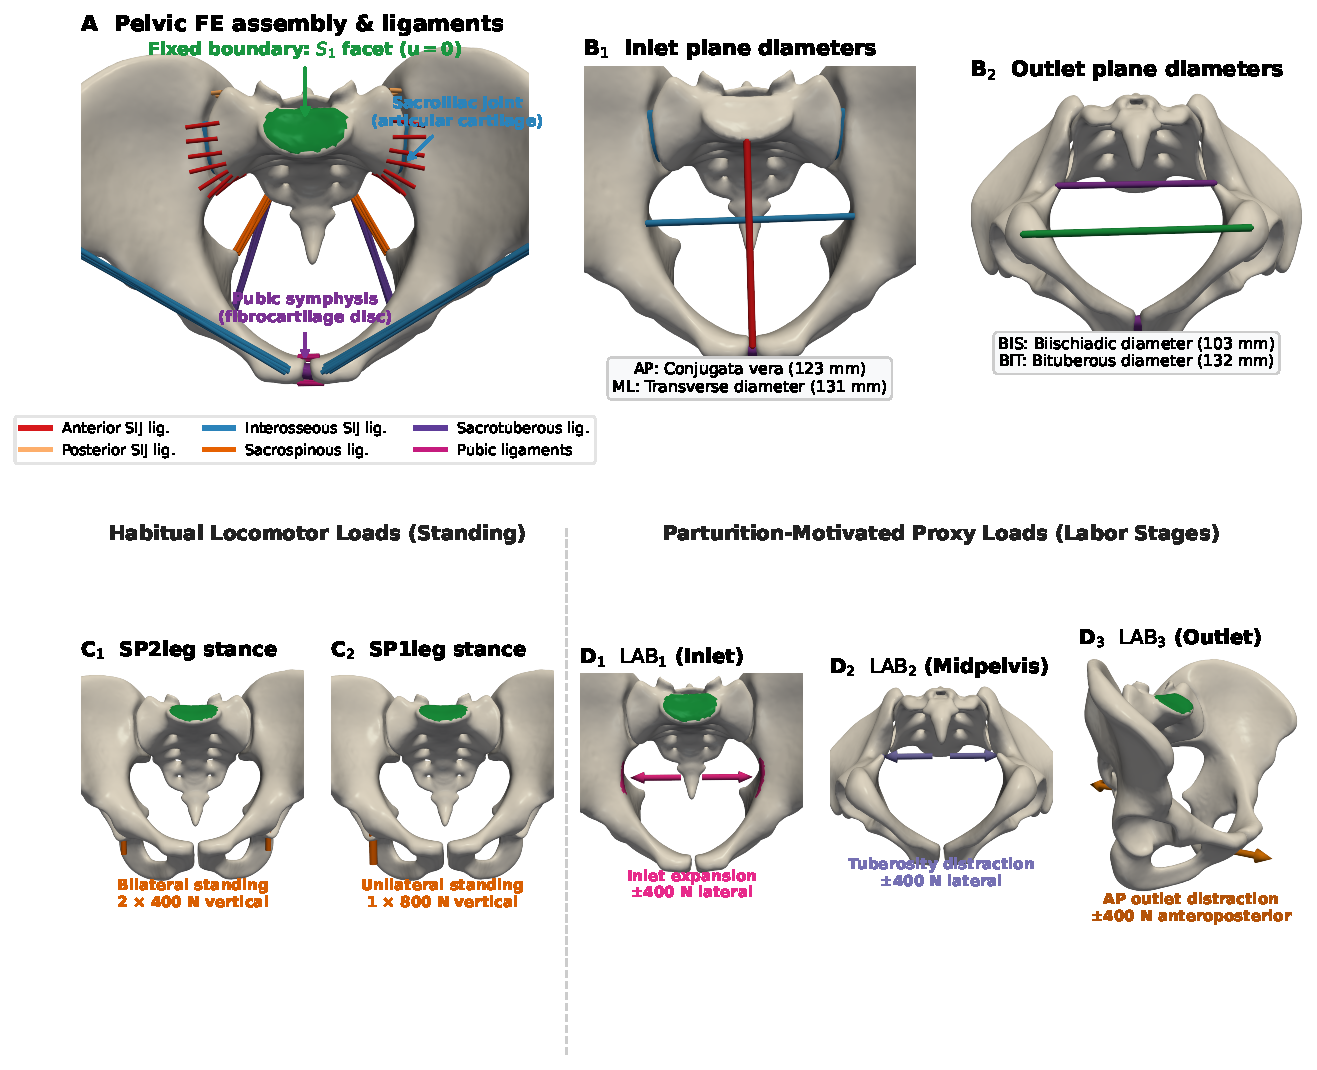
\includegraphics[width=0.95\linewidth]{images/model_setup.pdf}
  \caption{\textbf{Pelvic finite-element assembly, anatomical diameters, boundary conditions, and static load configurations.}
  (\textbf{A}) Complete 3D pelvic finite-element model comprising the sacrum, bilateral ossa coxae, sacroiliac joint (SIJ) articular cartilage (cyan), and pubic symphysis fibrocartilage disc (purple). Eleven discrete anatomical ligament bundles (anterior SIJ, posterior SIJ, interosseous SIJ, sacrospinous, sacrotuberous, and pubic ligaments) are explicitly represented. The superior articular surface of the sacrum ($S_1$ facet, green) is fixed against rigid-body displacement ($\mathbf{u} = \mathbf{0}$) via surface penalty.
  (\textbf{B}) True planar normal projections for anatomical pelvimetric diameters: ($\mathbf{B}_1$) pelvic inlet plane showing Conjugata vera (true conjugate, red, 123~mm) and transverse diameter (blue, 131~mm); ($\mathbf{B}_2$) pelvic outlet plane (inferior/perineal projection) showing biischiadic (interspinous) diameter (purple, 103~mm) and bituberous diameter (green, 132~mm).
  (\textbf{C}) Habitual locomotor load cases representing upright stance: ($\mathbf{C}_1$) bilateral standing ($\text{SP2leg}$, $2 \times 400\,\mathrm{N}$ vertical joint reaction forces applied at left and right acetabular notches); ($\mathbf{C}_2$) unilateral single-leg stance ($\text{SP1leg}$, $1 \times 800\,\mathrm{N}$ vertical joint reaction force applied at the right acetabulum).
  (\textbf{D}) Parturition-motivated proxy load cases representing stages of fetal transit through the pelvic canal: ($\mathbf{D}_1$) inlet ring expansion during head engagement ($\text{LAB}_1$, $\pm 400\,\mathrm{N}$ lateral expansion forces applied at the iliopectineal inner ring contacts); ($\mathbf{D}_2$) midpelvis transit ($\text{LAB}_2$, $\pm 400\,\mathrm{N}$ lateral distraction forces applied across the ischial tuberosities/spines); ($\mathbf{D}_3$) outlet clearance ($\text{LAB}_3$, $\pm 400\,\mathrm{N}$ anteroposterior distraction consisting of anterior traction on the pubic crest and posterior traction on the sacrococcygeal joint).}
  \label{fig:model-setup}
\end{figure}

\subsection{Pullback-assembled linear elasticity on a common reference domain}
\label{sec:pullback}

Let $\Omega_{\rm ref}\subset\mathbb R^3$ be the template domain and $\Omega_s$ the subject domain, related by a fixed diffeomorphic registration $x=\chi_s(X)$ with deformation gradient $F_s(X)=\nabla_X\chi_s(X)$ and Jacobian $J_s(X)=\det F_s>0$.
Writing $\chi_s(X)=X+\varphi_s(X)$, so $F_s=I+\nabla_X\varphi_s$, small-strain linear elasticity is solved on $\Omega_s$ but integrated on $\Omega_{\rm ref}$ through the standard change of variables~\citep{MarsdenHughes1983,BonetWood1997}.
For trial and test fields $\widehat{\mathbf u},\widehat{\mathbf v}\in V\subset[H^1(\Omega_{\rm ref})]^3$, the physical strain tensor at $x=\chi_s(X)$ is
\begin{equation}
\bm\varepsilon_x(\mathbf u)=\mathrm{sym}(\nabla_x \mathbf u)=\mathrm{sym}\!\big(\nabla_X \widehat{\mathbf u}\,F_s^{-1}\big),
\qquad
\bm\sigma_x=C_{\rm phys}(x):\bm\varepsilon_x(\mathbf u),
\end{equation}
and the pullback-assembled elastic bilinear form reads
\begin{equation}
a(\widehat{\mathbf u},\widehat{\mathbf v})
=\int_{\Omega_{\rm ref}}\!\Big[C_{\rm phys}\!\big(\chi_s(X)\big):\mathrm{sym}\!\big(\nabla_X \widehat{\mathbf u}\,F_s^{-1}\big)\Big]
:\mathrm{sym}\!\big(\nabla_X \widehat{\mathbf v}\,F_s^{-1}\big)\,J_s\,\mathrm dX.
\label{eq:pullback-bilinear}
\end{equation}
Here $F_s$ and $J_s$ arise only from the fixed image registration; no finite-strain mechanics is implied.
The mass bilinear form inherits the geometric volume factor,
\begin{equation}
m(\widehat{\mathbf u},\widehat{\mathbf v})
=\int_{\Omega_{\rm ref}} J_s(X)\,\widehat{\mathbf u}\cdot\widehat{\mathbf v}\,\mathrm dX,
\label{eq:mass-subject}
\end{equation}
defining an $L^2$ volume inner product weighted by local volumetric dilation rather than physical dynamic mass density.
The resulting generalised eigenvalues $\lambda_k = \boldsymbol\phi_k^\top K_s \boldsymbol\phi_k / (\boldsymbol\phi_k^\top M_s \boldsymbol\phi_k)$ quantify modal stiffness (or squared pseudo-frequencies), while the reciprocal eigenvalues $\lambda_k^{-1}$ describe modal compliance rather than physical resonance frequencies.
The \emph{unmapped} reference mass matrix $M_{\rm ref}^{0}$ is obtained from~\eqref{eq:mass-subject} with $J\equiv 1$ and provides a shared, registration-independent inner product across subjects.


\noindent\textbf{Material model.}
The physical elasticity tensor $C_{\rm phys}(x)$ is isotropic and heterogeneous.
For bone, the CT-derived hydroxyapatite density $\rho(x)$ is converted to ash density $\rho_{\mathrm{ash}}=(\rho+0.09)/1.14$ and mapped to a Young's modulus $E(x)$ via the Keller~\citep{Keller1994} piecewise power law,
\begin{equation}
E(x)=\begin{cases}
2398\,\mathrm{MPa}, & \rho_{\mathrm{ash}}(x)\le 0.486,\\[2pt]
\alpha\,\rho_{\mathrm{ash}}(x)^{\beta}, & \rho_{\mathrm{ash}}(x)>0.486,
\end{cases}
\qquad \alpha=10\,200,\ \beta=2.0,
\label{eq:keller}
\end{equation}
with Poisson's ratio $\nu=0.3$.
This family of density--modulus relations brackets published calibrations spanning the classical Carter--Hayes exponent~\citep{CarterHayes1977} and the site-dependent regressions of Morgan et al.~\citep{Morgan2003Trabecular}.
Cartilage (sacroiliac joints and pubic symphysis) is homogeneous linear elastic with $E=1.0$\,MPa and $\nu=0.45$.
These choices are consistent with structural adaptation and architecture--stiffness arguments in bone biomechanics~\citep{Frost1987,Huiskes1987,FarrKhosla2015,Zebaze2010Porosity} and with the broader sacroiliac and pubic-symphysis mechanics literature used to motivate linearised pelvic models~\citep{Snijders1993,Vleeming2012,Goode2008}.

\noindent\textbf{Ligaments in pullback coordinates.}
Ligament families are represented as polyline bundles mapped from template nodes $X_i$ to physical points $x_i=\chi_s(X_i)$.
For each segment $(X_i,X_j)$ define the physical unit tangent $\mathbf e=(x_j-x_i)/\|x_j-x_i\|$ and length $L=\|x_j-x_i\|$.
The total bundle stiffness and pretension are distributed across $N_{\rm seg}$ segments, yielding per-segment $k_{\rm seg}=K_{\rm bundle}/N_{\rm seg}$ and $T_{\rm seg}=T_{\rm bundle}/N_{\rm seg}$.
Each segment contributes an axial stiffness block
\begin{equation}
W=k_{\rm seg}\,(\mathbf e\mathbf e^\top),\qquad
K^{\rm ax}_{ij}=\begin{bmatrix} +W & -W\\ -W & +W\end{bmatrix},
\end{equation}
and, in the presence of pretension $T_{\rm seg}\ge 0$, a geometric (prestress) stiffness
\begin{equation}
K^{\rm geo}_{ij}=\tfrac{T_{\rm seg}}{L}\big(I-\mathbf e\mathbf e^\top\big)\succeq 0,
\label{eq:kgeo}
\end{equation}
together with paired nodal forces $\pm T_{\rm seg}\mathbf e$ on the right-hand side.
The full assembled tangent stiffness evaluated at the prestressed reference state is
\begin{equation}
K_s=K_{\rm elas,s}+K_{\rm lig,s}+K^{\rm geo}_s(T)+K_{\Gamma,s},\qquad
f=f_{\rm ext}+f_{\rm pret}(T),
\label{eq:K-assembled}
\end{equation}
where geometric stiffness $K^{\rm geo}_s(T)$ incorporates the stabilizing effect of initial ligament pretension $T$. In our linearised modal framework, incremental perturbations are evaluated directly about this prestressed configuration without requiring iterative non-linear equilibrium updates.
The term $K_{\Gamma,s}$ implements Dirichlet penalties on $\Gamma_{\rm ref}$,
$a_\Gamma(\widehat{\mathbf u},\widehat{\mathbf v})=\gamma\int_{\Gamma_{\rm ref}} \widehat{\mathbf u}\cdot\widehat{\mathbf v}\,J_{\Gamma,s}\,\mathrm dS_X$ with $J_{\Gamma,s}=J_s\|F_s^{-T}N\|$ and $\gamma=\alpha_\Gamma\bar E/h$, $\alpha_\Gamma\in[10^3,10^5]$.
A decade sweep of $\gamma$ left the reported cluster classification unchanged.

\noindent\textbf{Force-controlled loading.}
Neumann terms are pulled back to $\Gamma_{\rm ref}$ so that physical resultants are invariant under $\chi_s$:
\begin{equation}
\int_{\Gamma_s}\mathbf t_{\rm phys}\!\cdot\!\mathbf v\,\mathrm dS_x
=\int_{\Gamma_{\rm ref}} J_{\Gamma,s}(X)\,\mathbf t_{\rm phys}(\chi_s(X))\cdot\widehat{\mathbf v}(X)\,\mathrm dS_X.
\label{eq:neumann-pullback}
\end{equation}
All load cases in this study are defined by a total force $\mathbf F$ on a tagged physical region; the applied traction is $\mathbf t_{\rm phys}=\mathbf F/A_{\rm phys}$ with $A_{\rm phys}=\int_{\Gamma_{\rm ref}}J_{\Gamma,s}\,\mathrm dS_X$, so that $\int_{\Gamma_s}\mathbf t_{\rm phys}\,\mathrm dS_x=\mathbf F$ for every subject.

\subsection{Standardised load cases}
\label{sec:loading}

Loads were applied as force-controlled Neumann tractions via~\eqref{eq:neumann-pullback} so that every subject experienced the same integrated force vector regardless of physical surface area.
Two standing cases were considered: symmetric two-leg stance (SP2leg; $400$\,N per acetabulum, $+$CC) and one-leg stance (SP1leg; $800$\,N on the stance acetabulum, $+$CC).
The 400\,N per hip in SP2leg is a conservative split of head--arms--trunk mass onto both acetabula based on classical segment-inertia data~\citep{deLeva1996}, and the 800\,N one-leg value is well below in-vivo hip-implant peaks of 2.5--3.5$\times$BW recorded during single-leg support and gait~\citep{Bergmann2001JBiomech,Kutzner2016PLOS}.
Three proxy load cases probed parturition-relevant routing without modelling contact mechanics: \LABone\ applied bilateral mediolateral internal ring expansion forces ($\pm 400$\,N outward), \LABtwo\ applied bilateral ischial-tuberosity distraction ($\pm 400$\,N), and \LABthree\ applied anteroposterior outlet distraction between the pubis insertion ($-$AP, $400$\,N) and the sacrococcygeal joint ($+$AP, $400$\,N).
Their order of magnitude is consistent with published summaries of uterine contraction pressures of $\sim$40--80\,mmHg~\citep{AJOG2022Uterine,Mosby2012Pocket}, elevated intra-abdominal pressures during pregnancy~\citep{Fuchs2013PLOS,Chun2012IAPReview}, and review-level biomechanical estimates of fetal head--canal wall pressures during pushing~\citep{BiomechPregnancy2022}.
These loads are used as comparative probes rather than clinical simulations of labour~\citep{ChenGrimm2021,Almeida2024Uterus}.
The 400\,N and 800\,N force magnitudes act as standardized comparative probes of pelvic structural compliance. Static finite-element solutions solve the linear equilibrium equation $K_s \mathbf u = \mathbf f_{\rm ext} + \mathbf f_{\rm pret}(T)$, where $\mathbf f_{\rm pret}$ represents baseline ligament pretension ($20$\,N per ligament bundle) and $\mathbf f_{\rm ext}$ represents external load. By linearity, the displacement decomposes as $\mathbf u = \mathbf u_{\rm pret} + \delta\mathbf u_{\rm ext}$ with incremental external response $\delta\mathbf u_{\rm ext} = K_s^{-1}\mathbf f_{\rm ext}$. Scaling external force resultant $\mathbf f_{\rm ext} \to c\mathbf f_{\rm ext}$ scales incremental displacements strictly proportionally ($\delta\mathbf u_{\rm ext} \to c\,\delta\mathbf u_{\rm ext}$), such that modal expansion coefficients $q_i = \boldsymbol\phi_i^\top M_s \delta\mathbf u_{\rm ext}$ scale by $c$, modal energies $E_i = \frac{1}{2}\lambda_i q_i^2$ scale by $c^2$, and the normalized modal strain-energy fractions $f_i = E_i / \sum_j E_j$ of the incremental response are strictly invariant to load magnitude. Because external physiological loads ($400\text{--}800$\,N) substantially exceed baseline pretension, modal energy shares for total deformation remain approximately scale-invariant and are governed primarily by applied force geometry rather than magnitude.

\subsection{Generalised eigenproblem, rigid-mode filtering, and cross-subject pairing}
\label{sec:evp}

For each subject $s$ we assembled $(K_s,M_s)$ on $\Omega_{\rm ref}$ via~\eqref{eq:K-assembled} and~\eqref{eq:mass-subject} and solved the generalised eigenproblem
\begin{equation}
K_s\boldsymbol\phi_k=\lambda_k M_s\boldsymbol\phi_k,\qquad
\boldsymbol\phi_i^\top M_s \boldsymbol\phi_j=\delta_{ij},
\label{eq:gep}
\end{equation}
using a Krylov--Schur solver (SLEPc) with shift-invert spectral transform and MUMPS direct factorisation, extracting the $N_{\rm ev}=15$ lowest non-rigid eigenpairs.
Rigid modes (numerically $\lambda<10^{-8}$) were filtered.
For cross-subject comparison we used the mass-weighted modal assurance criterion on the shared reference metric,
\begin{equation}
\mathrm{MAC}_{M_0}(\mathbf x,\mathbf y)=
\frac{|\mathbf x^\top M_{\rm ref}^{0}\mathbf y|^2}
{(\mathbf x^\top M_{\rm ref}^{0}\mathbf x)(\mathbf y^\top M_{\rm ref}^{0}\mathbf y)}\in[0,1],
\label{eq:mac}
\end{equation}
and solved the Hungarian optimal-assignment problem on $-\mathrm{MAC}_{M_0}$ over the full $N_{\rm ev}\times N_{\rm ev}$ matrix~\citep{Kuhn1955Hungarian}, yielding an assignment bijection $\pi_s: \{1,\dots,N_{\rm ev}\} \to \{1,\dots,N_{\rm ev}\}$, where $\pi_s(i_{\rm ref}) = j_{\rm rank}$ maps reference identifier $i_{\rm ref}$ to its rank position in subject~$s$, and the inverse permutation $\pi_s^{-1}(j_{\rm rank}) = i_{\rm ref}$ assigns reference identity to each solver rank.
Entries with $\mathrm{MAC}_{M_0}<0.05$ were flagged as unpaired.
Rank index~$j$ (solver order) is required for gap statistics and cluster detection; the inverse assignment $\pi_s^{-1}(j)$ maps each solver mode back to its reference identity and is used only for anatomical interpretation, preserving the distinction between rank order and pathway identity emphasised in the Introduction.


\subsection{Spectral gap structure and clustered-regime detection}
\label{sec:gaps}

For each subject with ordered eigenvalues $\lambda_1\le\cdots\le\lambda_{N_{\rm ev}}$, relative consecutive gaps are
\begin{equation}
\mathrm{gap}_{\rm in}(i)=\frac{\lambda_{i+1}-\lambda_i}{\lambda_i},\qquad i=1,\ldots,N_{\rm ev}-1.
\label{eq:gap-in}
\end{equation}
A clustered regime $[i..j]$ is defined as the maximal contiguous rank block starting at~$i$ with internal gaps below threshold, $\mathrm{gap}_{\rm in}(k)<\varepsilon_{\rm in}$ for $k=i,\ldots,j-1$.
The threshold is set from data as the 25th percentile of the pooled $\mathrm{gap}_{\rm in}$ distribution across the cohort, yielding $\varepsilon_{\rm in}\approx 0.13$; sensitivity to the percentile choice is reported in Appendix~A.
External separation is quantified by
\begin{equation}
\mathrm{sep}_{\rm out}([i..j])=\min\!\left(\frac{\lambda_i-\lambda_{i-1}}{\lambda_i},\ \frac{\lambda_{j+1}-\lambda_j}{\lambda_j}\right),
\label{eq:sep-out}
\end{equation}
defined for interior clusters ($i > 1$ and $j < N_{\rm ev}$) where both adjacent neighbours exist. For boundary blocks reaching modal truncation (such as the 12--15 cluster with $N_{\rm ev}=15$), the upper neighbour is uncomputed and two-sided separation is formally undefined.
Exact mathematical multiplicity ($\lambda_i = \lambda_{i+1}$) was not observed under the operational numerical tolerance $\mathrm{gap}_{\rm in}\le\varepsilon_{\rm deg}=10^{-6}$ in any subject. While the absence of continuous or discrete spatial symmetries in the pelvic ring makes symmetry-enforced degeneracy impossible, it does not strictly preclude accidental parameter-dependent crossings; nonetheless, all regimes detected by~\eqref{eq:gap-in} are genuine near-degenerate clusters, for which small perturbations can drive rapid internal basis rotation and label exchange~\citep{Pierre1988,ManconiMace2017}.

\subsection{Invariant subspaces: principal angles, Grassmann distance, and Procrustes alignment}
\label{sec:subspace-methods}

For each clustered rank block of dimension~$r$, the corresponding subject-specific subspace was represented by an $M_{\rm ref}^{0}$-orthonormal basis
\begin{equation}
Q_s\in\mathbb R^{n\times r},\qquad Q_s^\top M_{\rm ref}^{0}\,Q_s=I_r.
\end{equation}
With a fixed reference basis $Q_{\rm ref}$, define the overlap matrix
\begin{equation}
S=Q_{\rm ref}^\top M_{\rm ref}^{0}\,Q_s\in\mathbb R^{r\times r},\qquad S=U\Sigma V^\top,\qquad \cos\theta_k=\sigma_k(S),
\label{eq:overlap}
\end{equation}
with singular values $\sigma_k$ yielding the principal angles $\theta_k\in[0,\pi/2]$ between the two subspaces~\citep{BjorckGolub1973Angles}.
The Grassmann distance is
\begin{equation}
d_G(Q_{\rm ref},Q_s)=\|\boldsymbol\theta\|_2=\Big(\sum_{k=1}^{r}\theta_k^2\Big)^{1/2}.
\label{eq:grassmann}
\end{equation}
When a stable basis representation inside a clustered subspace is required, we apply an orthogonal Procrustes rotation~\citep{Schoenemann1966Procrustes},
\begin{equation}
\widetilde Q_s=Q_s\,(V U^\top),
\label{eq:procrustes}
\end{equation}
which minimises the $M_{\rm ref}^{0}$-weighted distance $\|Q_{\rm ref} - Q_s R\|_{M_{\rm ref}^0}$ over orthogonal matrices $R\in\mathrm O(r)$ while preserving the subspace $\mathrm{span}(Q_s)$.

All quantitative biological comparisons use basis-invariant scalars derived from~\eqref{eq:overlap}--\eqref{eq:grassmann} or from the canonical-basis construction below.

\noindent\textbf{Degeneracy vs.\ near-degenerate mixing.}
Exact mathematical multiplicity requires $\lambda_i = \lambda_{i+1}$ (operationalized numerically as $\mathrm{gap}_{\rm in}(k)\le\varepsilon_{\rm deg}$ for all $k$ in the block, with $\varepsilon_{\rm deg}\ll\varepsilon_{\rm in}$); individual eigenvectors inside a degenerate subspace are then not unique, and any unitary rotation inside $\mathrm{span}(Q_s)$ is an equally valid basis.
When $\varepsilon_{\rm deg}<\mathrm{gap}_{\rm in}(k)<\varepsilon_{\rm in}$ the eigenvalues are close but distinct; the eigenvectors are formally unique, yet small perturbations can rotate the internal basis substantially while $\mathrm{span}(Q_s)$ itself remains nearly preserved.
This is the regime in which label exchange occurs without loss of the block-level mechanical content.

\subsection{Canonical anatomical functionals inside clustered subspaces}
\label{sec:canonical-methods}

To interpret clustered subspaces biologically, we use basis-invariant linear functionals defined by anatomical landmark pairs.
On the reference template mesh, five key obstetric and locomotor diameters are defined:
\begin{enumerate}[label=(\roman*)]
\item \textbf{AP inlet} ($s_{\rm AP}$): Promontory ($X_{\rm prom}$) to superior pubic symphysis ($X_{\rm pub}$), with unit direction $\mathbf e_{\rm AP} = (X_{\rm pub} - X_{\rm prom}) / \|X_{\rm pub} - X_{\rm prom}\|$;
\item \textbf{ML inlet} ($s_{\rm ML}$): Widest transverse diameter across left and right iliopectineal lines ($X_{\rm left}, X_{\rm right}$), with unit direction $\mathbf e_{\rm ML} = (X_{\rm right} - X_{\rm left}) / \|X_{\rm right} - X_{\rm left}\|$;
\item \textbf{Biischiadic outlet} ($s_{\rm BIS}$): Left to right ischial spine ($X_{\rm sp,left}, X_{\rm sp,right}$), with unit direction $\mathbf e_{\rm BIS} = (X_{\rm sp,right} - X_{\rm sp,left}) / \|X_{\rm sp,right} - X_{\rm sp,left}\|$;
\item \textbf{Bituberous outlet} ($s_{\rm BIT}$): Left to right inferior ischial tuberosity ($X_{\rm tub,left}, X_{\rm tub,right}$), with unit direction $\mathbf e_{\rm BIT} = (X_{\rm tub,right} - X_{\rm tub,left}) / \|X_{\rm tub,right} - X_{\rm tub,left}\|$;
\item \textbf{AP outlet} ($s_{\rm OUTLETAP}$): Sacrococcygeal joint ($X_{\rm cocc}$) to inferior pubic symphysis ($X_{\rm pub,inf}$), with unit direction $\mathbf e_{\rm OUTAP} = (X_{\rm pub,inf} - X_{\rm cocc}) / \|X_{\rm pub,inf} - X_{\rm cocc}\|$.
\end{enumerate}
For each subject $s$, patient-specific landmark coordinates follow the registration mapping $X^s = X + \boldsymbol\varphi_s(X)$, and the resulting functional observable for a displacement field $\mathbf u$ is
\begin{equation}
s_\ell^{(s)}(\mathbf u) = \mathbf e_\ell^{(s)\top}\! \big(\mathbf u(X_{\rm target}^s) - \mathbf u(X_{\rm origin}^s)\big) = \mathbf b_\ell^{(s)\top}\mathbf u, \qquad \ell \in \{\text{AP, ML, BIS, BIT, OUTLETAP}\},
\label{eq:functional-score}
\end{equation}
with measurement vectors $\mathbf b_\ell^{(s)} \in \mathbb R^n$ constructed using inverse-distance weighting (IDW) interpolation onto the $k_{\rm idw}=8$ nearest mesh nodes around each anatomical landmark coordinate, ensuring smooth, mesh-robust landmark displacement estimates across subjects.

\noindent\textbf{Basis-invariant single-functional capacity.}
For any individual functional $\mathbf b_\ell^{(s)}$ and an $M_{\rm ref}^0$-orthonormal basis $Q_s \in \mathbb R^{n \times r}$ spanning a clustered subspace of dimension $r$ ($Q_s^\top M_{\rm ref}^0 Q_s = I_r$), every displacement in the subspace is parameterized by $\mathbf u = Q_s \boldsymbol\alpha$ with $\boldsymbol\alpha \in \mathbb R^r$.
The maximum functional response attainable over the unit modal sphere $\|\boldsymbol\alpha\|_2 \le 1$ is:
\begin{equation}
\kappa_\ell(Q_s) = \max_{\|\boldsymbol\alpha\|_2 \le 1} \mathbf b_\ell^{(s)\top} Q_s \boldsymbol\alpha = \|Q_s^\top \mathbf b_\ell^{(s)}\|_2.
\label{eq:single-functional-norm}
\end{equation}
This extremal capacity is achieved along the unique modal direction $\boldsymbol\alpha^* = Q_s^\top \mathbf b_\ell^{(s)} / \|Q_s^\top \mathbf b_\ell^{(s)}\|_2$, defining the optimal spatial displacement field:
\begin{equation}
\boldsymbol\psi_\ell^{(s)} = Q_s \frac{Q_s^\top \mathbf b_\ell^{(s)}}{\|Q_s^\top \mathbf b_\ell^{(s)}\|_2} \in \mathbb R^n.
\label{eq:single-functional-field}
\end{equation}
Under an arbitrary internal basis rotation $\widetilde Q_s = Q_s R$ with $R \in \mathrm O(r)$, we have
\begin{equation}
\|\widetilde Q_s^\top \mathbf b_\ell^{(s)}\|_2 = \|R^\top Q_s^\top \mathbf b_\ell^{(s)}\|_2 = \|Q_s^\top \mathbf b_\ell^{(s)}\|_2 = \kappa_\ell(Q_s),
\end{equation}
and the physical displacement field transforms identically:
\begin{equation}
\widetilde{\boldsymbol\psi}_\ell^{(s)} = (Q_s R) \frac{R^\top Q_s^\top \mathbf b_\ell^{(s)}}{\|R^\top Q_s^\top \mathbf b_\ell^{(s)}\|_2} = Q_s R R^\top \frac{Q_s^\top \mathbf b_\ell^{(s)}}{\|Q_s^\top \mathbf b_\ell^{(s)}\|_2} = \boldsymbol\psi_\ell^{(s)}.
\end{equation}
Both the scalar capacity $\kappa_\ell(Q_s)$ and the physical displacement field $\boldsymbol\psi_\ell^{(s)}$ are therefore strictly invariant under any internal orthogonal basis rotation, providing an objective, single-functional measure that requires no bivariate coordinate choices.
The corresponding normalized coupling score is reported in millimetres of diameter change per millimetre of maximum nodal modal displacement:
\begin{equation}
\widehat\kappa_\ell^{(s)} = \frac{|\mathbf b_\ell^{(s)\top}\boldsymbol\psi_\ell^{(s)}|}{\max_a \|\boldsymbol\psi_{\ell,a}^{(s)}\|_2}.
\label{eq:single-coupling-score}
\end{equation}

\noindent\textbf{Multivariate canonical decomposition.}
When joint coupling across a pair of measurement vectors $(\mathbf b_1^{(s)}, \mathbf b_2^{(s)})$ (e.g., AP and ML inlet, or BIS and BIT outlet) is examined, we assemble the covector matrix $B_s = [\mathbf b_1^{(s)}\ \ \mathbf b_2^{(s)}] \in \mathbb R^{n \times 2}$ and its subspace projection:
\begin{equation}
C_s = Q_s^\top B_s = \big[Q_s^\top\mathbf b_1^{(s)}\ \ Q_s^\top\mathbf b_2^{(s)}\big] \in \mathbb R^{r \times 2}, \qquad C_s = U_s \Sigma_s V_s^\top,
\label{eq:canonical-proj}
\end{equation}
where the singular values $\sigma_1 \ge \sigma_2$ quantify joint extremal capacities.
The canonical displacement modes in physical space are $\boldsymbol\psi_k^{(s)} = Q_s U_s[:, k]$ ($k=1, 2$), with corresponding dual functionals in covector space $\widetilde{\mathbf b}_k^{(s)} = B_s V_s[:, k] = V_s[0, k]\mathbf b_1^{(s)} + V_s[1, k]\mathbf b_2^{(s)}$.
By construction, their action is exactly equal to the singular values: $\widetilde{\mathbf b}_k^{(s)\top}\boldsymbol\psi_k^{(s)} = \sigma_k$.
The clean singular scores normalized by maximum nodal displacement are $\widehat s_k^{(s)} = \sigma_k / \max_a \|\boldsymbol\psi_{k,a}^{(s)}\|_2$.
Because $V_s \in \mathrm O(2)$ mixes the two anatomical axes, mode $\boldsymbol\psi_1^{(s)}$ is primary-dominant only when $|V_s[0, 0]| \ge |V_s[1, 0]|$; across the pelvic cohort, the first singular mode in the 9--10 subspace is predominantly aligned with the higher-compliance transverse (ML) axis ($|V_s[1, 0]| > |V_s[0, 0]|$ in $99.6\%$ of subjects).
For unambiguous, axis-specific evaluation of anatomical opening without coordinate mixing, the basis-invariant single-functional capacity $\widehat\kappa_\ell^{(s)}$ (Eq.~\ref{eq:single-coupling-score}) serves as our primary quantitative metric, while joint-SVD scores provide complementary bivariate structure.

\subsection{Whole-pelvis global deformation pattern decomposition}
\label{sec:mechanisms-methods}

We analysed the fifteen stored reference eigenvectors on the complete reference continuum mesh, without anatomical subdivision.
Continuous displacement fields were sampled using positive 14-point tetrahedral quadrature (exact for polynomials up to degree~4; Basix scheme), ensuring exact numerical integration of products between piecewise-linear finite-element fields ($P_1$) and quadratic polynomial templates ($P_2$, degree~3) as well as quadratic-quadratic products ($P_2 \times P_2$, degree~4).
Direct projection onto local strain fields $\boldsymbol\varepsilon_k=\tfrac12(\nabla\mathbf u_k+\nabla\mathbf u_k^\top)$ leaves 97--99\% of the strain norm in the residual across all eigenmodes, because compliance and strain concentrate heavily in the cartilaginous joints (sacroiliac joints and pubic symphysis).
This localized joint concentration masks global ring deformation and fails to discriminate modes.
To recover the global ring-level character, we evaluate overall shape change across the entire pelvic continuum.

Infinitesimal rigid-body motion (3 translations and 3 rotations) is spanned by the 6-parameter field $\mathbf u_{\rm rigid}(\mathbf x)=\mathbf t+\boldsymbol\omega\times(\mathbf x-\mathbf x_c)$, where $\mathbf x_c=\langle\mathbf x\rangle_V$ is the volume-weighted centroid.
The volume-weighted rigid design matrix was orthonormalised via reduced QR decomposition ($\mathbf Q_{\rm rigid}$), and rigid motion was projected out from the displacement field:
\begin{equation}
\mathbf u_{\rm nonrigid} = \mathbf u - \mathbf Q_{\rm rigid}(\mathbf Q_{\rm rigid}^\top \mathbf u).
\end{equation}
Rigid rotation is therefore completely eliminated upfront and is not one of the reported deformation categories.

Coordinates relative to the centroid $\mathbf x_c$ were scaled by the gyration radius $r_g = \sqrt{\langle \|\mathbf x - \mathbf x_c\|^2 \rangle_V}$, defining normalised coordinates $(\tilde x, \tilde y, \tilde z) = (\mathbf x - \mathbf x_c)/r_g$ in the anatomical frame (ML, AP, CC).
Rather than conditioning on an artificial 1D beam axis, the deformation is decomposed across the entire 3D ring into four canonical deformation families spanning the complete 24-dimensional nonrigid polynomial displacement space up to quadratic order:
\begin{enumerate}[label=(\roman*)]
\item \textbf{Axial} (6~DOF): uniform normal extension/compression and normal strain gradients along all three axes,
$u_i \in \operatorname{span}\{\tilde x_i, \tfrac12 \tilde x_i^2\}$ for $i \in \{x, y, z\}$;
\item \textbf{Bending} (6~DOF): pure Euler-Bernoulli flexural modes with zero shear strain ($\varepsilon_{ij} = 0$ for $i \ne j$),
$\mathbf b_{ij} = \tfrac12 \tilde x_i^2 \mathbf e_j - \tilde x_i \tilde x_j \mathbf e_i$ for each ordered pair $i \ne j \in \{x, y, z\}$;
\item \textbf{Shear} (10~DOF): uniform transverse shears ($( \tilde y, \tilde x, 0 )$, $( 0, \tilde z, \tilde y )$, $( \tilde z, 0, \tilde x )$), six quadratic transverse shear gradients, and the complete irrotational quadratic shear mode $\mathbf w = \nabla(\tilde x \tilde y \tilde z) = (\tilde y \tilde z, \tilde x \tilde z, \tilde x \tilde y)^\top$ ($d=10$ total);
\item \textbf{Torsion} (2~DOF): Saint-Venant twist gradients with zero normal strain,
$\mathbf t_x = (0, -\tilde x \tilde z, \tilde x \tilde y)^\top$ and $\mathbf t_y = (\tilde y \tilde z, 0, -\tilde x \tilde y)^\top$.
\end{enumerate}
Templates in each family were projected orthogonal to $\mathbf Q_{\rm rigid}$ and orthonormalised using reduced singular value decomposition.
The combined 24-dimensional nonrigid basis $\mathbf A$ spans the deformation space with low condition number ($\kappa(\mathbf A) \approx 4.58$ on the reference pelvis), corresponding to a Gram matrix condition number $\kappa(\mathbf G) = \kappa(\mathbf A)^2 \approx \GramConditionNumber$.
Because the four deformation families have intrinsic mathematical overlap on irregular geometries, Shapley value allocation is employed as an objective game-theoretic method to partition the explained squared nonrigid norm fairly and symmetrically across the overlapping subspaces, rather than acting as a separator of mutually orthogonal physical mechanisms:
\begin{equation}
f_m = \sum_{S \subseteq M \setminus \{m\}} \frac{|S|!(|M|-|S|-1)!}{|M|!} \left[ R^2(S \cup \{m\}) - R^2(S) \right], \qquad
\sum_{m=1}^4 f_m + f_{\rm residual} = 1,
\end{equation}
where $R^2(S)$ is the fraction of nonrigid squared norm explained by subspace subset $S$, and $f_{\rm residual} = 1 - R^2(M)$.
Shapley allocation distributes the explained squared norm without order-dependent orthogonalisation bias.
The fractions are invariant to eigenvector sign and amplitude, describe a specified global 3D shape-change model, and are not strain-energy shares.
Comprehensive mathematical derivations of the continuum inner product, 14-point tetrahedral quadrature, canonical polynomial dictionary, cooperative game-theoretic Shapley allocation, numerical conditioning, synthetic backward-recovery benchmarks, and complete 15-mode quantitative profiles are detailed in Appendix~E (Tables~E1--E2).

\subsection{Load routing and modal strain-energy fractions}
\label{sec:routing-methods}

For each load case we solved the static problem $K_s\mathbf u_s=\mathbf b$ on $\Omega_{\rm ref}$, projected the result onto the $M_s$-orthonormal eigenbasis $\Phi$,
\begin{equation}
q=\Phi^\top M_s\mathbf u_s,\qquad E_i=\tfrac12\lambda_i q_i^2,\qquad f_i=\frac{E_i}{\sum_{j=1}^{N_{\rm ev}} E_j},
\label{eq:modal-fraction}
\end{equation}
and summarised each pathway's contribution by its retained modal strain-energy fraction $f_i$ evaluated across the $N_{\rm ev}=15$ computed modes.
Block throughput for a clustered regime $C$ is $f_C=\sum_{i\in C}f_i$, and the dominant mode set $N_{80}$ of a load case is the smallest subset of modes (selected in descending order of mean energy contribution) whose cumulative mean energy fractions reach at least 0.80.
For cross-load comparison we also report cosine similarity of full 15-mode mean profiles and Jaccard overlap of dominant mode sets.


\subsection{First-order eigenvalue sensitivities and analytical uncertainty propagation}
\label{sec:sensitivities}

To propagate material-parameter uncertainty to the spectrum without repeated finite-element solves, we use classical first-order sensitivities of the generalised eigenproblem~\eqref{eq:gep}: for a parameter $p_j$ that affects only the stiffness,
\begin{equation}
\frac{\partial\lambda_m}{\partial p_j}
=\frac{\boldsymbol\phi_m^\top\,(\partial K_s/\partial p_j)\,\boldsymbol\phi_m}
{\boldsymbol\phi_m^\top M_s\,\boldsymbol\phi_m}.
\label{eq:ev-sensitivity}
\end{equation}
For ligament parameters, $\partial K_s/\partial k_{\rm seg}=\mathbf e\mathbf e^\top$ and $\partial K_s/\partial T_{\rm seg}=(I-\mathbf e\mathbf e^\top)/L$ are aggregated over segments in each bundle using the geometric assembly underlying~\eqref{eq:kgeo}.
For cartilage moduli, $\partial K_s/\partial E_{\rm region}$ is the element-wise elastic stiffness integrated over the corresponding joint domain, scaled by the baseline modulus.
For the high-density branch of~\eqref{eq:keller}, the chain rule gives $\partial E/\partial\alpha=E/\alpha$ and $\partial E/\partial\beta=E\ln\rho_{\rm ash}$, integrated over the bone domain.
Storing the dimensionless Jacobians
\begin{equation}
J_j^{(m)}=\frac{p_j}{\lambda_m}\frac{\partial\lambda_m}{\partial p_j}
\end{equation}
once per subject lets us compute first-order log-space variance propagation as $\mathrm{Var}(\log\lambda_m) \approx \mathbf J_m^\top \Sigma_{\log p} \mathbf J_m$ for any prior covariance $\Sigma_{\log p} = \mathrm{Cov}(\log\mathbf p)$ on the material parameters, including hierarchical priors that separate global, per-type, and left/right components.
For adjacent eigenvalues $\lambda_i, \lambda_{i+1}$, the variance of the gap $\Delta\lambda = \lambda_{i+1}-\lambda_i$ is computed from the combined sensitivity vector $\mathbf g_{i,i+1} = \lambda_{i+1}\mathbf J_{i+1} - \lambda_i\mathbf J_i$ as
\begin{equation}
\mathrm{Var}(\lambda_{i+1}-\lambda_i) \approx \mathbf g_{i,i+1}^\top \Sigma_{\log p}\,\mathbf g_{i,i+1} \approx \mathrm{Var}(\lambda_{i+1}) + \mathrm{Var}(\lambda_i) - 2\,\mathrm{Cov}(\lambda_i, \lambda_{i+1}),
\label{eq:gap-cov}
\end{equation}
accounting for the substantial positive covariance induced by shared tissue parameters.
Fig.~\ref{fig:material-uq} summarises the resulting variance decomposition across the 15 lowest eigenvalues and the covariance-aware gap signal-to-noise ratio across solver ranks.
For the low-rank backbone (modes~1--3), adjacent gap signal-to-noise ratios remain high ($Z \gg 1.0$), demonstrating that modal ordering is gap-protected against material uncertainty.
In contrast, for the 9--10 inlet cluster, the gap signal-to-noise ratio drops below unity ($Z < 1.0$, Fig.~\ref{fig:material-uq}B), indicating that the nominal spectral gap is comparable to predicted material-parameter uncertainty, consistent with local label exchangeability.
Cluster boundaries and subspace definitions remain well-defined under the posited parameter covariances, reinforcing that the compact subspace, rather than the isolated modal label, is the robust physical object.
Full hierarchical priors, Shapley-style decompositions, and sex-stratified versions are reported in Appendix~B and Appendix~D.

\begin{figure}[!htbp]
  \centering
  \includegraphics[width=\linewidth]{../../analysis_outputs/plos_revision/figures/material_uncertainty.pdf}
  \caption{\textbf{Analytical propagation of material-parameter uncertainty to eigenvalues and spectral gaps.}
  \textbf{(A)} Total coefficient of variation (CoV, \%) of eigenvalues $\lambda_1,\ldots,\lambda_{15}$ under hierarchical material-parameter covariance, stratified by sex (blue: male; yellow: female).
  \textbf{(B)} Relative gap signal-to-noise ratio (spectral gap divided by propagated standard deviation) between adjacent solver ranks, incorporating shared-parameter covariance $\mathrm{Cov}(\lambda_i, \lambda_{i+1})$.
  The shaded region highlights the 9--10 rank transition. Triangles mark 10th-percentile values across subjects.}
  \label{fig:material-uq}
\end{figure}

\subsection{Decomposition of variability sources and robustness analyses}
\label{sec:robustness-methods}

To separate shape and material contributions to spectral variability, we compared the full cohort against a shape-only cohort ($\chi_s$, fixed reference bone modulus) and a material-only cohort (identity deformation, subject-specific bone modulus).
Robustness was assessed by (i)~random permutation of subject order (invariance to machine precision), (ii)~subject bootstrap with replacement ($N{=}278$, 500 replicates) with threshold re-estimation, alongside random 80\% subsampling for cohort stability, and (iii)~morphology-axis permutation null tests in which a one-dimensional anatomical proxy $\mu$ (e.g.\ AP inlet diameter) was shuffled 1000 times to assess whether swap-rate localisation along $\mu$ exceeded chance (Table~A6).
Post-hoc allometric regressions of $\log\lambda_k$ on isotropic body-size scale~$s$ (with instrumental variables from volume, surface, and mass) and Shapley/LMG variance decomposition into scale, sex, shape, and material contributions are reported in Appendix~D.

\subsection{Minimal analytical model for the near-degenerate regime}
\label{sec:toy-methods}

The cluster/subspace framework admits a compact analytical interpretation via a two-degree-of-freedom model.
Let $q_1,q_2$ denote two generalised rotational coordinates and define a stiffness matrix
\begin{equation}
K_2=\begin{bmatrix} k_1 & c\\ c & k_2\end{bmatrix},\qquad \Delta=k_1-k_2,\qquad k_1,k_2>0,\ k_1k_2>c^2,
\end{equation}
with detuning~$\Delta$ and coupling~$c$.
The eigenvalues are
\begin{equation}
\lambda_{\pm}=\frac{k_1+k_2}{2}\pm\sqrt{\Big(\tfrac{\Delta}{2}\Big)^2+c^2},
\qquad
\tan(2\theta)=\frac{2c}{\Delta},
\label{eq:2dof-eig}
\end{equation}
and the minimum separation $\lambda_+-\lambda_-=2|c|$ is attained at $\Delta=0$, where the mixing angle passes through $\pi/4$ and the modes exchange character.
The operational criterion
\begin{equation}
|\Delta(\mu)|\le\tau\,|c(\mu)|\quad\text{for some morphology parameter }\mu,\qquad \tau\in[1.5,2],
\label{eq:2dof-criterion}
\end{equation}
separates near-degenerate/mixing from stable-ordering regimes.
Adding a third coordinate $q_3$ with stiffness~$s$ and coupling vector $\mathbf d = [d_1, d_2]^\top$, dynamic reduction of the $3\times 3$ eigenproblem $(K - \lambda I)\mathbf q = \mathbf 0$ gives the exact non-linear reduced eigenproblem
\begin{equation}
\Big( K_2 - \frac{\mathbf d \mathbf d^\top}{s - \lambda} \Big) \mathbf q_{12} = \lambda \mathbf q_{12}.
\label{eq:dynamic-schur}
\end{equation}
In the low-frequency limit ($\lambda \ll s$), static condensation yields the linear effective stiffness
\begin{equation}
K_{\rm eff} = K_2 - \frac{\mathbf d \mathbf d^\top}{s} = \begin{bmatrix} k_1-d_1^2/s & c-d_1d_2/s\\ c-d_1d_2/s & k_2-d_2^2/s\end{bmatrix},
\label{eq:schur}
\end{equation}
showing how a compliant hidden pathway (small~$s$) shifts effective detuning and coupling and pushes a system toward an avoided crossing veering region.
In all stochastic numerical simulations (Fig.~\ref{fig:toy}), the full $3\times 3$ eigenproblem is solved directly without static or dynamic truncation.
In the $n$-DOF finite-element setting, the detected clusters correspond to $\{q_1,q_2\}$, the canonical basis $(\boldsymbol\psi_1,\boldsymbol\psi_2)$ to the rotated eigenvectors, and $\mathrm{gap}_{\rm in}$ to $(\lambda_+-\lambda_-)/\lambda_-$.
A stochastic population instantiation of this model, shown and discussed in Fig.~\ref{fig:toy} and Sec.~\ref{sec:toy-results}, reproduces the label--subspace dissociation, the standing-vs-task routing contrast, and the effect of hidden-pathway variability observed in the full pelvic cohort.
Explicit derivations, the small-$c$ expansion, and the full stochastic population extension are provided in Appendix~D.

\subsection{Statistical analysis}
\label{sec:statistics}

All statistical analyses were executed using SciPy, statsmodels, and custom Python routines.
Continuous metrics across non-normal cohorts were evaluated using non-parametric methods.
Two-group comparisons (e.g., non-swapped vs.\ swapped cluster members, or male vs.\ female distributions) were conducted using two-sided Mann--Whitney $U$ tests.
Effect sizes for Mann--Whitney tests are reported as rank-biserial correlations, $r_{\rm rb} = 1 - 2U / (n_1 n_2) \in [-1, 1]$, and Cliff's $\delta$.
Paired differences across loading conditions or mode pairs were assessed via two-sided Wilcoxon signed-rank tests.
Bivariate associations between continuous anatomical dimensions (such as AP inlet diameter or isotropic scale) and modal metrics (energy fractions, spectral gaps) were quantified using Spearman's rank correlation coefficient $\rho_s$.
Multiple hypothesis testing across spectral ranks and loading cases was controlled using the Benjamini--Hochberg procedure, maintaining the false discovery rate at $q < 0.05$; adjusted $p$-values are reported where indicated.
Confidence intervals for median differences and effect sizes were obtained via bias-corrected and accelerated (BCa) bootstrap resampling ($10\,000$ resamples).
Cohort-level cluster stability was evaluated by repeating the detection pipeline across 500 random subcohorts of 80\% sample size drawn without replacement ($n = 222$), yielding 95\% subsampling stability intervals.
Full population inference was additionally confirmed by resampling subjects with replacement ($N = 278$, 500 replicates) with end-to-end recalculation of the cluster threshold $\varepsilon_{\rm in}$.

Differences in subspace orientation across the cohort were quantified using the Grassmann distance $d_G(Q_{\rm ref}, Q_s) = \|\boldsymbol\theta\|_2$.
Importantly, $d_G$ measures the intrinsic geometric distance between the linear subspaces $\mathrm{span}(Q_{\rm ref})$ and $\mathrm{span}(Q_s)$ in the Grassmannian manifold $\mathrm{Gr}(r, n)$, which is strictly invariant to arbitrary unitary rotations of the internal basis within either subspace.
Consequently, population variations in $d_G$ (such as sex-specific differences) represent true rotations of the subspace orientation within $\mathbb R^n$, rather than artefacts of internal basis re-indexing.

\subsection{Software and computational implementation}


Finite-element assembly, eigensolves, and postprocessing were implemented in Python~3.11 with DOLFINx/FEniCSx~($\ge$0.10), PETSc, and SLEPc.
All reported figures, tables, and numerical values are produced by scripts included in the study repository.
Results are stored as compressed Zarr arrays for reproducible downstream analysis.
Further implementation details, dependency versions, and reproduction instructions are provided in the appendices and the code repository.

% ============================================================
\section*{Data availability}
Derived summary data supporting the findings of this study are provided within the manuscript, the appendices, and the study repository.
The standardised pelvic geometries originate from the BoneDat research dataset~\citep{HenyssKuchar2025BoneDat}; access to the underlying clinical imaging data remains subject to source-data governance restrictions and requires approval through the procedures described in the dataset publication.

\section*{Code availability}
Custom code used to assemble the models, run the spectral analyses, and generate the reported figures and tables is available in the study repository.
A public archival release of the analysis code will accompany publication.

\section*{Author contributions}
P.H.,\ M.K.,\ and N.H.\ conceptualised the study.
P.H.\ and M.K.\ developed the computational models and performed the simulations.
P.H.,\ M.K.,\ and A.M.\ analysed the data.
P.H.,\ M.K.,\ A.M.,\ and N.H.\ interpreted the results and wrote the manuscript.
All authors reviewed and approved the final manuscript.

\section*{Competing interests}
The authors declare no competing interests.

\section*{Acknowledgments}
We thank the BoneDat project for curating the standardised imaging-derived dataset used in this study.

\clearpage
\appendix

\section{Spectral cluster architecture}

The Supporting Information appendices collect detailed robustness, specificity, and model-boundary analyses that support the findings presented in the main text.

This appendix expands the bookkeeping behind the recurrent clustered regimes, including reference-mode occupancy, swap frequencies, and morphology-axis diagnostics.
Table~A1 reproduces the cohort-level cluster list used in the main Results.
Table~A2 records the mapping between recurrent rank clusters and their dominant reference-mode identities.
Table~A3 reports per-mode swap rates, Table~A4 gives the adjacent rank-pair diagnostics, Table~A5 summarises the exchange-regime classification, and Table~A6 reports the morphology-axis permutation null test used to localise swap behaviour.

\subsection*{Table A1. Detected near-degenerate rank clusters}
\SuppTableInput{../../analysis_outputs/tables/clusters.tex}

\subsection*{Table A2. Rank-cluster to reference-mode mapping}
\SuppTableInput{../../analysis_outputs/tables/rank_cluster_ref_mapping.tex}

\subsection*{Table A3. Per-mode swap rates}
\SuppTableInput{../../analysis_outputs/tables/swap_rates.tex}

\subsection*{Table A4. Adjacent rank-pair swap diagnostics}
\SuppTableInput{../report/swap_pair_diagnostics.tex}

\subsection*{Table A5. Cluster-level exchange classification}
\SuppTableInput{../report/veering_vs_mixing_classification.tex}

\subsection*{Table A6. Morphology-axis permutation null test}
\SuppTableInput{../../analysis_outputs/tables/veering_null_test.tex}

\clearpage
\section{Cohort robustness and sex effects}

The main text uses sex effects only where they materially sharpen interpretation of the recurrent clustered subspaces, especially the 9--10 inlet-related pair.
This appendix provides the broader sex-stratified summary and the subsampling stability evidence that the dominant clusters are stable cohort-level features rather than products of a few outlying subjects.
Table~B1 gives the subsampling stability estimates for the dominant clusters and gap statistics.
Figure~B1 summarises the sex-stratified spectral structure, and Table~B2 reports the accompanying sex-stratified statistical tests for the spectral and subspace metrics.

\subsection*{Table B1. Subsampling stability under random 80\% subcohorts}
\SuppTableInput{../../analysis_outputs/tables/cohort_bootstrap_robustness.tex}

\subsection*{Figure B1. Sex-stratified spectral summary}
\begin{center}
  \includegraphics[width=\linewidth]{../../analysis_outputs/figures/sex_stratified_summary.pdf}
\end{center}

\subsection*{Table B2. Sex-stratified tests for spectral and subspace metrics}
\SuppTableInput{../../analysis_outputs/tables/sex_stratified_summary.tex}

\clearpage
\section{Load-routing specificity}

The main manuscript uses standing and proxy childbirth loads to show the contrast between a robust low-rank backbone and selectively recruited higher-rank subspaces.
This appendix provides comprehensive load-specificity diagnostics, including cluster-level function-locking, dominant-mode sets, and pairwise overlap of full routing profiles.

Figure~C1 visualises the load--function locking map across the prevalent clusters.
Table~C1 summarises the phase-specific coupling synthesis, Table~C2 reproduces the dominant mode-set summary used in the main text for appendix-level completeness, and Table~C3 reports the pairwise overlap metrics for the full load-routing profiles.

\subsection*{Figure C1. Load-function coupling heatmap across prevalent clusters}
\begin{center}
  \includegraphics[width=\linewidth]{../../analysis_outputs/figures/function_locking_heatmap.pdf}
\end{center}

\subsection*{Table C1. Load-function coupling synthesis}
\SuppTableInput{../../analysis_outputs/tables/function_locking_synthesis.tex}

\subsection*{Table C2. Dominant mode sets for standing and proxy loading}
\SuppTableInput{../../analysis_outputs/tables/mode_activation_dominant_sets.tex}

\subsection*{Table C3. Pairwise overlap of load-routing profiles}
\SuppTableInput{../../analysis_outputs/tables/mode_activation_overlap.tex}

\clearpage
\section{Model-boundary and sensitivity analyses}

These analyses bound the main claims rather than extend them.
Allometry quantifies what is lost when the main spectral analysis is performed on size-normalised pelves.
Material uncertainty quantifies how much absolute eigenvalue identifiability would degrade under broader soft-tissue and density-law scatter while showing that the relative fragile-versus-robust gap architecture is preserved.
Figure~D1 shows the post-hoc allometric recovery analysis, and Table~D1 summarises the corresponding scaling exponents and variance decomposition.
Figure~D2 presents the threshold sensitivity, reference sensitivity, isotropic scale vs solver gap, and 15-mode displacement reconstruction error, alongside Table~D2 which tabulates the combined first-order uncertainty propagation used to support the robustness discussion in the main text.

\subsection*{Figure D1. Allometry dashboard}
\begin{center}
  \includegraphics[width=\linewidth]{../../analysis_outputs/figures/allometry_dashboard.pdf}
\end{center}

\clearpage

\subsection*{Table D1. Allometry summary}
\input{../../analysis_outputs/tables/allometry_summary.tex}

\clearpage

\subsection*{Figure D2. Robustness and reconstruction dashboard}
\begin{center}
  \includegraphics[width=\linewidth]{../../analysis_outputs/plos_revision/figures/robustness.pdf}
\end{center}

\clearpage

\subsection*{Table D2. Combined first-order material uncertainty summary}
\input{../../analysis_outputs/material_uncertainty/material_uncertainty_table.tex}

\clearpage
\section{Whole-pelvis 3D canonical deformation pattern decomposition}
\label{sec:appendix-global-deformation}

This appendix provides the complete mathematical formulation, continuum quadrature proofs, coordinate transformations, canonical polynomial dictionary, cooperative game-theoretic projection mechanics, numerical conditioning diagnostics, and synthetic backwards-identification benchmarks for the whole-pelvis 3D deformation decomposition presented in Section~\ref{sec:atlas-results} and Figure~\ref{fig:modes-atlas}.
Table~E1 tabulates the complete 15-mode quantitative profile across all four canonical deformation families, standalone $R^2$ values, and residual fractions.
Table~E2 reports the synthetic benchmark validations across idealized symmetric and irregular pelvic domains.

\subsection{Physical motivation: Cartilage compliance concentration vs.\ ring-level kinematics}
The pelvic ring is a closed, doubly-curved structural biomechanical loop composed of three major bony segments (the sacrum and bilateral coxal bones) joined anteriorly at the pubic symphysis and posteriorly at the bilateral sacroiliac joints (SIJs).
In continuum mechanics, the standard approach to characterise modal kinematics would be to evaluate the infinitesimal Cauchy strain tensor field,
\begin{equation}
\boldsymbol\varepsilon(\mathbf u) = \tfrac{1}{2}\big(\nabla \mathbf u + \nabla \mathbf u^\top\big).
\label{eq:cauchy-strain}
\end{equation}
However, while physiological dynamic elastic moduli of articular cartilage and symphyseal fibrocartilage are frequently reported in the range $E_{\rm cartilage} \sim 10\text{--}50\,\mathrm{MPa}$, in our quasi-static equilibrium finite-element formulations an effective relaxed equilibrium modulus of $E_{\rm cartilage} = \CartilageEffectiveModulus\,\mathrm{MPa}$ is prescribed for the sacroiliac cartilage cleft and pubic symphysis disc.
This effective modulus accounts for sustained equilibrium compliance across the pelvic syndesmoses, which are three to four orders of magnitude more compliant than cortical and trabecular bone ($E_{\rm bone} \sim 5\text{--}18\,\mathrm{GPa}$).
Under generalised modal vibration, elastic deformation naturally channels into these narrow compliant interfaces.
Consequently, direct $L^2$-projection of the Cauchy strain field onto low-order polynomial strain templates leaves between 97\% and 99\% of the strain norm unexplained in the residual across all fifteen computed eigenmodes.
The intense local strain spikes in the millimeter-thin joint clefts completely overpower and conceal the systemic, ring-scale kinematics (such as whole-pelvis flaring, torsion, and inlet/outlet dilation).

Furthermore, modeling the human pelvis as a one-dimensional beam conditioned along an arbitrary anatomical axis (e.g., mediolateral, anteroposterior, or craniocaudal) imposes an unphysical 1D kinematic constraint on a closed, three-dimensional ring.
For complex three-dimensional deformation pathways involving coupled out-of-plane flexure and transverse shearing (such as Mode~2), 1D axis conditioning artificially drives the unexplained residual up to 84\%, distorting biological interpretation.
To overcome both limitations, our framework evaluates the overall shape change across the entire three-dimensional pelvic continuum without anatomical partitioning and without imposing artificial 1D beam axes, removing infinitesimal rigid-body motion upfront before decomposing the remaining shape change into four canonical 3D polynomial deformation families.

\subsection{Continuum inner product and 14-point tetrahedral quadrature}
Let $\Omega \subset \mathbb{R}^3$ denote the reference pelvic continuum domain with volume $V = \int_\Omega \mathrm{d}V$.
The natural inner product on the displacement space $[L^2(\Omega)]^3$ weighted by volume is
\begin{equation}
\langle \mathbf u, \mathbf v \rangle_V = \frac{1}{V} \int_\Omega \mathbf u(\mathbf x) \cdot \mathbf v(\mathbf x) \, \mathrm{d}V, \qquad
\|\mathbf u\|_V^2 = \langle \mathbf u, \mathbf u \rangle_V.
\label{eq:volume-inner-product}
\end{equation}
The continuous reference domain $\Omega$ is discretized into an unstructured tetrahedral mesh $\mathcal{T}_h = \{K_e\}_{e=1}^{N_e}$ using piecewise-linear ($P_1$) Lagrange continuous finite elements.
Within any tetrahedron $K$, a $P_1$ displacement field $\mathbf u_h(\mathbf x)$ is an affine vector function of position ($\mathbf u_h|_K \in \mathcal{P}_1(K)$).
When computing projections against quadratic deformation modes $\mathbf p_2 \in \mathcal{P}_2(K)$, the modal cross-product integrand $\mathbf u_h \cdot \mathbf p_2$ is a cubic polynomial ($\mathcal{P}_3(K)$), and the dictionary Gram matrix integrand $\mathbf p_2 \cdot \mathbf p_2$ is a quartic polynomial ($\mathcal{P}_4(K)$).
Standard 4-point linear tetrahedral quadrature rules (precision degree 2) incur quadrature truncation errors when integrating degree-3 and degree-4 polynomials.

To evaluate all continuum inner products with exact polynomial precision and zero quadrature truncation error, we employ a symmetric, positive degree-4 tetrahedral quadrature rule with 14 points per tetrahedron (constructed via Basix).
For each tetrahedron $K$, the 14 quadrature points $\mathbf x_{K,q}$ and strictly positive weights $w_{K,q} > 0$ satisfy $\sum_{q=1}^{14} w_{K,q} = |K|$ and integrate all polynomials up to degree 4 exactly:
\begin{equation}
\int_K p(\mathbf x) \, \mathrm{d}V = \sum_{q=1}^{14} w_{K,q} \, p(\mathbf x_{K,q}) \qquad \forall p \in \mathcal{P}_4(K).
\end{equation}
Summing across all $N_e$ tetrahedra gives $N_q = 14 N_e$ discrete sampling points with weights $w_p > 0$.
Defining normalized quadrature weights $\tilde w_p = w_p / \sum_{j=1}^{N_q} w_j$, the continuum inner product~\eqref{eq:volume-inner-product} is evaluated with exact numerical precision:
\begin{equation}
\langle \mathbf u, \mathbf v \rangle_V = \sum_{p=1}^{N_q} \tilde w_p \, \mathbf u(\mathbf x_p) \cdot \mathbf v(\mathbf x_p).
\label{eq:quadrature-sum}
\end{equation}

\subsection{Infinitesimal rigid-body motion elimination}
Infinitesimal rigid-body displacements in $\mathbb{R}^3$ constitute a 6-dimensional linear Lie algebra subspace $\mathfrak{se}(3)$ consisting of 3 translations and 3 rotations:
\begin{equation}
\mathbf u_{\rm rigid}(\mathbf x) = \mathbf t + \boldsymbol\omega \times (\mathbf x - \mathbf x_c), \qquad \mathbf t, \boldsymbol\omega \in \mathbb{R}^3,
\label{eq:rigid-field}
\end{equation}
where $\mathbf x_c$ is the volume-weighted spatial centroid of the pelvic domain,
\begin{equation}
\mathbf x_c = \langle \mathbf x \rangle_V = \sum_{p=1}^{N_q} \tilde w_p \, \mathbf x_p.
\end{equation}
To ensure scale-free, dimensionally consistent kinematics across subjects, we define the reference gyration radius $r_g$ and non-dimensionalised anatomical coordinates $\tilde{\mathbf x} = (\tilde x, \tilde y, \tilde z)^\top$:
\begin{equation}
r_g = \sqrt{\langle \|\mathbf x - \mathbf x_c\|^2 \rangle_V} = \sqrt{\sum_{p=1}^{N_q} \tilde w_p \|\mathbf x_p - \mathbf x_c\|^2}, \qquad
\tilde{\mathbf x} = \frac{\mathbf x - \mathbf x_c}{r_g}.
\label{eq:dimless-coords}
\end{equation}
Here the Cartesian coordinate directions correspond to the standard anatomical axes: $x$ is mediolateral (ML), $y$ is anteroposterior (AP), and $z$ is craniocaudal (CC).

In the discrete quadrature representation, each displacement field is a stacked vector $\mathbf U \in \mathbb{R}^{3N_q}$ with components $U_{3p-3+i} = \sqrt{\tilde w_p} \, u_i(\mathbf x_p)$ for $i \in \{1,2,3\}$.
The 6 rigid-body design modes $\mathbf r_1, \dots, \mathbf r_6 \in \mathbb{R}^{3N_q}$ (corresponding to unit translations along $x,y,z$ and unit infinitesimal rotations about $x,y,z$) form the rigid design matrix $\mathbf R \in \mathbb{R}^{3N_q \times 6}$.
We compute its thin QR decomposition,
\begin{equation}
\mathbf R = \mathbf Q_{\rm rigid} \mathbf R_{\rm upper}, \qquad \mathbf Q_{\rm rigid} \in \mathbb{R}^{3N_q \times 6}, \quad \mathbf Q_{\rm rigid}^\top \mathbf Q_{\rm rigid} = \mathbf I_6.
\end{equation}
The orthogonal projection operator onto the nonrigid displacement subspace is then:
\begin{equation}
\mathbf P_{\rm nonrigid} = \mathbf I_{3N_q} - \mathbf Q_{\rm rigid} \mathbf Q_{\rm rigid}^\top.
\label{eq:nonrigid-proj}
\end{equation}
For any raw modal displacement field $\mathbf u$, the nonrigid component is $\mathbf u_{\rm nonrigid} = \mathbf P_{\rm nonrigid} \mathbf u$, and the total squared displacement norm partitions orthogonally:
\begin{equation}
\|\mathbf u\|_V^2 = \|\mathbf u_{\rm rigid}\|_V^2 + \|\mathbf u_{\rm nonrigid}\|_V^2, \qquad
f_{\rm nonrigid} = \frac{\|\mathbf u_{\rm nonrigid}\|_V^2}{\|\mathbf u\|_V^2}.
\end{equation}
Crucially, rigid rotation is eliminated at this foundational stage: it is neither retained in the target deformation field nor reported as an explained deformation category.
If a displacement field satisfies $\|\mathbf u_{\rm nonrigid}\|_V^2 / \|\mathbf u\|_V^2 \le 10^{-20}$, it is identified as a pure rigid motion and excluded from nonrigid decomposition.

\subsection{Canonical 3D polynomial dictionary}
The vector space of polynomial displacement fields $\mathbf u(\tilde{\mathbf x})$ of degree at most 2 in three dimensions has complete algebraic dimension $3 \times \binom{3+2}{2} = \TotalPolyDOFs$.
Subtracting the \RigidDOFs\ degrees of freedom of infinitesimal rigid motion leaves an exact \NonrigidDOFs-dimensional nonrigid polynomial quotient space.
We decompose this space into four canonical physical deformation families spanning all \NonrigidDOFs\ nonrigid degrees of freedom:
\begin{enumerate}[label=(\roman*)]
\item \textbf{Axial family ($d_{\rm axial} = 6$ degrees of freedom):}
Uniform normal extension/compression along each anatomical axis, together with quadratic normal strain gradients:
\begin{equation}
\begin{aligned}
\mathbf a_{x,1} &= (\tilde x, 0, 0)^\top, &\quad \mathbf a_{x,2} &= (\tfrac{1}{2}\tilde x^2, 0, 0)^\top, \\
\mathbf a_{y,1} &= (0, \tilde y, 0)^\top, &\quad \mathbf a_{y,2} &= (0, \tfrac{1}{2}\tilde y^2, 0)^\top, \\
\mathbf a_{z,1} &= (0, 0, \tilde z)^\top, &\quad \mathbf a_{z,2} &= (0, 0, \tfrac{1}{2}\tilde z^2)^\top.
\end{aligned}
\label{eq:axial-family}
\end{equation}

\item \textbf{Bending family ($d_{\rm bending} = 6$ degrees of freedom):}
Classical pure Euler-Bernoulli flexural modes.
For any pair of distinct coordinate axes $i \ne j \in \{x, y, z\}$, the displacement field
\begin{equation}
\mathbf b_{ij} = \tfrac{1}{2}\tilde x_i^2 \mathbf e_j - \tilde x_i \tilde x_j \mathbf e_i
\label{eq:bending-family}
\end{equation}
satisfies $\partial_i u_j = \tilde x_i$ and $\partial_j u_i = -\tilde x_i$.
Consequently, the Cauchy shear strain vanishes identically:
\begin{equation}
\varepsilon_{ij}(\mathbf b_{ij}) = \tfrac{1}{2}\big(\partial_j u_i + \partial_i u_j\big) = \tfrac{1}{2}\big(-\tilde x_i + \tilde x_i\big) \equiv 0.
\end{equation}
The six ordered pairs $(x,y)$, $(x,z)$, $(y,x)$, $(y,z)$, $(z,x)$, $(z,y)$ thus define six independent shear-free flexural modes.

\item \textbf{Shear family ($d_{\rm shear} = 10$ degrees of freedom):}
Comprises three uniform transverse shears, six planar quadratic transverse shear gradients, and one triaxial cross-gradient shear field $\mathbf w$:
\begin{equation}
\begin{aligned}
\mathbf s_{xy,1} &= (\tilde y, \tilde x, 0)^\top, &\quad \mathbf s_{xy,2} &= (\tilde x \tilde y, \tfrac{1}{2}\tilde x^2, 0)^\top, &\quad \mathbf s_{yx,2} &= (\tfrac{1}{2}\tilde y^2, \tilde y \tilde x, 0)^\top, \\
\mathbf s_{yz,1} &= (0, \tilde z, \tilde y)^\top, &\quad \mathbf s_{yz,2} &= (0, \tilde y \tilde z, \tfrac{1}{2}\tilde y^2)^\top, &\quad \mathbf s_{zy,2} &= (0, \tfrac{1}{2}\tilde z^2, \tilde z \tilde y)^\top, \\
\mathbf s_{zx,1} &= (\tilde z, 0, \tilde x)^\top, &\quad \mathbf s_{zx,2} &= (\tfrac{1}{2}\tilde z^2, 0, \tilde z \tilde x)^\top, &\quad \mathbf s_{xz,2} &= (\tilde x \tilde z, 0, \tfrac{1}{2}\tilde x^2)^\top, \\
\mathbf w &= (\tilde y \tilde z, \tilde x \tilde z, \tilde x \tilde y)^\top = \nabla(\tilde x \tilde y \tilde z).
\end{aligned}
\label{eq:shear-family}
\end{equation}
Unlike bending, these modes produce non-zero shear strains $\varepsilon_{ij} \ne 0$.
The triaxial mode $\mathbf w$ is irrotational ($\nabla \times \mathbf w = \mathbf 0$) and divergence-free ($\nabla \cdot \mathbf w = 0$), uniquely completing the \NonrigidDOFs-dimensional nonrigid polynomial quotient.

\item \textbf{Torsion family ($d_{\rm torsion} = 2$ degrees of freedom):}
Saint-Venant torsional twist gradients around the three Cartesian axes:
\begin{equation}
\mathbf t_x = (0, -\tilde x \tilde z, \tilde x \tilde y)^\top, \quad
\mathbf t_y = (\tilde y \tilde z, 0, -\tilde x \tilde y)^\top, \quad
\mathbf t_z = (-\tilde y \tilde z, \tilde x \tilde z, 0)^\top.
\label{eq:torsion-family}
\end{equation}
Each torsion field exhibits identically zero normal strain ($\varepsilon_{xx} = \varepsilon_{yy} = \varepsilon_{zz} \equiv 0$).
Crucially, these three vector fields satisfy the identity:
\begin{equation}
\mathbf t_x + \mathbf t_y + \mathbf t_z \equiv \mathbf 0.
\end{equation}
Hence, the space of Saint-Venant torsional twist has algebraic dimension exactly equal to 2, spanned by $\{\mathbf t_x, \mathbf t_y\}$.
\end{enumerate}

To assemble the discrete kinematic design matrix, the basis fields in each family $m \in \{\text{axial, bending, shear, torsion}\}$ are sampled at the $N_q$ quadrature points, weighted by $\sqrt{\tilde w_p}$, projected orthogonal to $\mathbf Q_{\rm rigid}$ via $\mathbf P_{\rm nonrigid}$, and orthonormalised via reduced singular value decomposition (SVD):
\begin{equation}
\mathbf P_{\rm nonrigid} \mathbf A_m = \mathbf Q_m \mathbf \Sigma_m \mathbf V_m^\top, \qquad \mathbf Q_m \in \mathbb{R}^{3N_q \times d_m}, \quad \mathbf Q_m^\top \mathbf Q_m = \mathbf I_{d_m}.
\end{equation}
The concatenated design matrix $\mathbf A = [\mathbf Q_{\rm axial}, \mathbf Q_{\rm bending}, \mathbf Q_{\rm shear}, \mathbf Q_{\rm torsion}] \in \mathbb{R}^{3N_q \times \NonrigidDOFs}$ spans the complete \NonrigidDOFs-dimensional canonical nonrigid deformation subspace.

\subsection{Numerical conditioning, family overlap, and the Gram matrix}
It is important to note that the four canonical deformation families have intrinsic algebraic overlap and are not mutually orthogonal even on an idealized symmetric domain.
For example, on the symmetric unit cube $[-1, 1]^3$ (volume $V = 8$), the unnormalized continuum volume integral between the bending mode $\mathbf b = (-xy, \frac{1}{2}x^2, 0)^\top$ and the shear mode $\mathbf s = (xy, \frac{1}{2}x^2, 0)^\top$ evaluates analytically to $\int_{[-1, 1]^3} \mathbf b \cdot \mathbf s \, \mathrm dV = -22/45 \approx -0.4889$, corresponding to a volume-normalized inner product $\langle \mathbf b, \mathbf s \rangle_V = \frac{1}{V}\int_{[-1, 1]^3} \mathbf b \cdot \mathbf s \, \mathrm dV = -11/180 \approx -0.0611$ (angular cosine $\cos\theta = -11/29 \approx -0.3793$).
Consequently, the four deformation families share non-zero algebraic overlap by mathematical necessity, independently of geometric irregularity.

On the real, geometrically asymmetric pelvic ring, this intrinsic algebraic overlap combines with anatomical geometry.
The kinematic design matrix $\mathbf A$ has 2-norm condition number $\kappa(\mathbf A) \approx \DesignConditionNumber$, and the associated Gram matrix $\mathbf G = \mathbf A^\top \mathbf A \in \mathbb{R}^{\NonrigidDOFs \times \NonrigidDOFs}$ has condition number:
\begin{equation}
\kappa(\mathbf G) = \frac{\sigma_{\max}(\mathbf G)}{\sigma_{\min}(\mathbf G)} = \kappa(\mathbf A)^2 \approx \GramConditionNumber.
\end{equation}
A Gram condition number of $\sim 21$ confirms that all \NonrigidDOFs\ canonical modes remain linearly independent and well-conditioned without numerical rank deficiency.

\subsection{Cooperative game-theoretic Shapley value norm allocation}
Because the four deformation subspaces have intrinsic mathematical overlap and cannot be mutually orthogonal, projecting onto them sequentially (e.g., Gram-Schmidt orthogonalisation) would introduce an arbitrary, order-dependent bias: the first chosen family would absorb all shared variance, artificially starving subsequent families.
To achieve an objective, order-independent decomposition, we formulate the problem using cooperative game theory.

Let $M = \{\text{axial}, \text{bending}, \text{shear}, \text{torsion}\}$ denote the set of four pattern players ($|M| = 4$).
There are $2^4 = 16$ possible coalitions $S \subseteq M$.
For any coalition $S$, we construct the concatenated family design matrix $\mathbf A_S \in \mathbb{R}^{3N_q \times \sum_{m \in S} d_m}$ and define the characteristic function $v(S)$ as the fraction of nonrigid squared displacement norm explained by the joint subspace:
\begin{equation}
v(S) = R^2(S) = \frac{\mathbf u_{\rm nonrigid}^\top \mathbf P_S \mathbf u_{\rm nonrigid}}{\|\mathbf u_{\rm nonrigid}\|_V^2}, \qquad
\mathbf P_S = \mathbf A_S (\mathbf A_S^\top \mathbf A_S)^+ \mathbf A_S^\top,
\label{eq:coalition-r2}
\end{equation}
with $v(\emptyset) = 0$, where $(\cdot)^+$ denotes the Moore-Penrose pseudoinverse.
The Shapley value $f_m$ assigned to each deformation family $m \in M$ is the unique allocation satisfying the four foundational Shapley axioms:
\begin{enumerate}
\item \textbf{Efficiency:} The sum of allocated values equals the value of the grand coalition:
\begin{equation}
\sum_{m \in M} f_m = v(M) = R^2(M) = 1 - f_{\rm residual}.
\end{equation}
\item \textbf{Symmetry:} If two families $m, k \in M$ contribute identically to every coalition ($v(S \cup \{m\}) = v(S \cup \{k\})$ for all $S \subseteq M \setminus \{m, k\}$), then $f_m = f_k$.
\item \textbf{Dummy player:} If a family $m$ adds zero marginal variance to every coalition ($v(S \cup \{m\}) = v(S)$ for all $S \subseteq M \setminus \{m\}$), then $f_m = 0$.
\item \textbf{Additivity:} If a deformation field is decomposed into independent orthogonal components, their Shapley shares sum linearly.
\end{enumerate}
The explicit Shapley allocation formula evaluates the marginal contribution of family $m$ averaged over all coalition orders:
\begin{equation}
f_m = \sum_{S \subseteq M \setminus \{m\}} \frac{|S|!(|M| - |S| - 1)!}{|M|!} \Big[ v\big(S \cup \{m\}\big) - v(S) \Big].
\label{eq:shapley-formula}
\end{equation}
The unexplained shape change is retained as an explicit residual:
\begin{equation}
f_{\rm residual} = 1 - v(M) = 1 - R^2(\text{axial} \cup \text{bending} \cup \text{shear} \cup \text{torsion}).
\end{equation}
Because subspace projection operators are monotonic ($V_S \subseteq V_{S \cup \{m\}} \implies v(S \cup \{m\}) \ge v(S)$), every marginal contribution is non-negative, which guarantees $f_m \ge 0$ for all $m$.
Exact closure holds identically:
\begin{equation}
f_{\rm axial} + f_{\rm bending} + f_{\rm shear} + f_{\rm torsion} + f_{\rm residual} \equiv 1.0000 \quad (100.0\%).
\end{equation}
Furthermore, the fractions are strictly scale-invariant ($\mathbf u \mapsto c\mathbf u$ for $c \ne 0$) and sign-invariant ($\mathbf u \mapsto -\mathbf u$).
For comparative diagnostics, we also compute the standalone coefficient of determination for each isolated family:
\begin{equation}
R^2_m = v(\{m\}) = \frac{\mathbf u_{\rm nonrigid}^\top \mathbf P_m \mathbf u_{\rm nonrigid}}{\|\mathbf u_{\rm nonrigid}\|_V^2}.
\end{equation}
Due to the intrinsic geometric coupling between families ($\kappa(\mathbf G) \approx \GramConditionNumber$), the sum $\sum_{m \in M} R^2_m$ may moderately exceed the total explained fraction $R^2(M)$; the Shapley values partition this shared overlap fairly and symmetrically.

\subsection{Synthetic benchmark and backwards-identification validation}
To verify the accuracy, robustness, and backwards-identifiability of the global deformation decomposition, we executed synthetic validation experiments on both an idealized symmetric domain (cube) and the realistic reference pelvis mesh (Table~E2).

On the symmetric domain, pure synthetic fields belonging to the axial, shear, and torsion families are identified with $100.0\%$ fidelity, zero cross-talk, and exactly $0.0\%$ residual.
For pure Euler-Bernoulli bending ($\mathbf u = (-xy, \tfrac{1}{2}x^2, 0)$), the displacement field consists of an axial cross-term $-xy$ and a transverse parabolic deflection $\tfrac{1}{2}x^2$.
Because the quadratic shear mode $\mathbf s_{xy,2} = (xy, \tfrac{1}{2}x^2, 0)$ shares the identical transverse parabolic deflection $\tfrac{1}{2}x^2$, the pure flexural field lies in the joint span $V_{\rm bending} \oplus V_{\rm shear}$.
The Shapley allocation splits this shared transverse deflection analytically, yielding $77.5\%$ bending, $22.5\%$ shear, and exactly $0.0\%$ residual ($100.0\%$ fitted).

On the actual reference pelvis mesh, pure canonical polynomial fields are recovered with exactly $0.0\%$ residual ($100.0\%$ fitted fraction):
\begin{itemize}
\item Pure axial stretch ($x\mathbf e_x$): $85.3\%$ axial share, $0.0\%$ residual ($100.0\%$ fitted).
\item Pure triaxial extension ($x\mathbf e_x - \tfrac{1}{2}y\mathbf e_y - \tfrac{1}{2}z\mathbf e_z$): $84.8\%$ axial share, $0.0\%$ residual ($100.0\%$ fitted).
\item Pure Euler-Bernoulli bending: $74.1\%$ bending share, $0.0\%$ residual ($100.0\%$ fitted).
\item Pure transverse shear: $82.8\text{--}90.7\%$ shear share, $0.0\%$ residual ($100.0\%$ fitted).
\item Pure Saint-Venant torsion: $91.3\text{--}97.7\%$ torsion share, $0.0\%$ residual ($100.0\%$ fitted).
\end{itemize}
When subjected to pure infinitesimal rigid translations or pure infinitesimal rotations, the nonrigid fraction is detected as $f_{\rm nonrigid} < 10^{-27}$, correctly triggering the rigid-motion filter and confirming zero spurious contamination.
Finally, adding arbitrary rigid-body translations and rotations to an axial deformation field yields identical Shapley shares ($85.3\%$ axial, $7.2\%$ bending, $7.5\%$ shear, $0.0\%$ torsion, $0.0\%$ residual) to within machine precision ($< 10^{-10}$), demonstrating complete invariance under rigid-body frame shifts.

\subsection{Reference mode deformation profiles and biomechanical interpretation}
Table~E1 compiles the quantitative whole-pelvis 3D deformation decomposition for all fifteen reference eigenmodes.
The results resolve several key biomechanical features of the pelvic ring:
\begin{itemize}
\item \textbf{Modes~1 and~2 (low-rank backbone):}
For Mode~1, the nonrigid deformation accounts for $3.3\%$ of the total displacement norm (the remainder reflecting whole-pelvis rocking on the sacroiliac/pubic supports).
Its nonrigid shape change is predominantly out-of-plane torsional twist ($22.7\%$) and transverse shear ($17.7\%$), with a total fitted fraction of $42.7\%$ (residual $57.3\%$).
For Mode~2, nonrigid shape change ($5.5\%$ of total norm) is a coupled sagittal ring flexure and shear ($23.6\%$ bending, $23.7\%$ shear, $20.8\%$ axial, $68.6\%$ fitted, residual $31.4\%$).
This resolves the earlier 1D beam artifact (which had yielded an unphysical $84\%$ residual): the true 3D ring kinematics explain more than two-thirds of the deformation norm.

\item \textbf{Modes~4 and~5 (dominant flexural pathways):}
Modes~4 and~5 exhibit strong bending dominance, explaining $43.6\%$ and $47.4\%$ of their nonrigid norm respectively (with standalone bending fits $R^2_{\rm bending}$ reaching $47.6\%$ and $62.4\%$, and total explained fractions of $74.4\%$ and $86.3\%$).
These modes capture lateral and anteroposterior flaring of the iliac wings.

\item \textbf{The obstetric 9--10 pair:}
Mode~9 is the most highly fitted mode in the entire spectrum ($91.8\%$ explained, residual only $8.2\%$).
Its deformation is overwhelmingly axial ($60.6\%$ Shapley share; standalone $R^2_{\rm axial} = 67.7\%$), representing circumferential normal stretching that widens the obstetric pelvic inlet.
In contrast, its near-degenerate partner Mode~10 ($74.9\%$ fitted) is dominated by shear ($35.2\%$) and torsion ($34.3\%$), with minimal axial contribution ($4.3\%$; standalone $R^2_{\rm torsion} = 30.3\%$, $R^2_{\rm shear} = 32.7\%$, residual $25.1\%$).
This quantitative kinematic divergence reinforces why the 9--10 cluster forms a complementary functional unit: Mode~9 provides direct obstetric diameter enlargement, whereas Mode~10 accommodates asymmetric torsional/shear loads.
\end{itemize}

\clearpage
\subsection*{Table E1. Reference mode whole-pelvis 3D deformation decomposition}
\SuppTableInput{../../analysis_outputs/tables/global_deformation_modes_table.tex}

\clearpage
\subsection*{Table E2. Synthetic benchmark and backwards-identification validation}
\SuppTableInput{../../analysis_outputs/tables/global_deformation_synthetic_table.tex}

\clearpage
\bibliographystyle{unsrtnat}






\bibliography{../report/references}

\end{document}
